\documentclass[10pt,a4paper,openany]{report}

%==================================
% CODIFICACIÓN, IDIOMA Y TIPOGRAFÍA
%==================================

\usepackage[utf8]{inputenc}
\usepackage[T1]{fontenc}
\usepackage[spanish,es-nodecimaldot]{babel}
\usepackage{lmodern}
\usepackage{microtype}

%==================================
% PAQUETES GENERALES
%==================================

\usepackage{graphicx}
\usepackage{float}
\usepackage{geometry}
\usepackage{array}
\usepackage{booktabs}
\usepackage{tabularx}
\usepackage{longtable}
\usepackage{ragged2e}
\usepackage{enumitem}
\usepackage{titlesec}
\usepackage{setspace}
\usepackage{fancyhdr}
\usepackage{caption}
\usepackage{needspace}

%==================================
% BIBLIOGRAFÍA CON BIBLATEX Y BIBER
%==================================

\usepackage[autostyle=true,spanish=mexican]{csquotes}

\usepackage[
backend=biber,
style=ieee,
citestyle=numeric-comp,
sorting=none,
isbn=false,
doi=true,
url=true
]{biblatex}

\addbibresource{referencias.bib}

% Hyperref debe cargarse después de biblatex
\usepackage[hidelinks]{hyperref}

%==================================
% MÁRGENES Y ÁREA DE TEXTO
%==================================

\geometry{
	a4paper,
	left=3.5cm,
	right=3.5cm,
	top=2.3cm,
	bottom=2.5cm,
	headheight=14pt,
	headsep=0.45cm,
	footskip=1cm
}

%==================================
% TEXTO Y PÁRRAFOS
%==================================

\setstretch{1.0}
\setlength{\parindent}{0pt}
\setlength{\parskip}{3pt}
\setlength{\emergencystretch}{2em}
\setlist[itemize]{topsep=3pt,itemsep=2pt,parsep=0pt,partopsep=0pt}
\setlist[enumerate]{topsep=3pt,itemsep=2pt,parsep=0pt,partopsep=0pt}

%==================================
% FORMATO DE CAPÍTULOS Y SECCIONES
%==================================

\titleformat{\chapter}[hang]
{\normalfont\bfseries\Large}
{\thechapter}
{1em}
{}

\titlespacing*{\chapter}
{0pt}
{-15pt}
{10pt}

\titleformat{\section}
{\normalfont\bfseries\large}
{\thesection}
{0.7em}
{}

\titlespacing*{\section}
{0pt}
{10pt}
{4pt}

\titleformat{\subsection}
{\normalfont\bfseries\normalsize}
{\thesubsection}
{0.7em}
{}

\titlespacing*{\subsection}
{0pt}
{8pt}
{3pt}

%==================================
% ENCABEZADO Y PIE DE PÁGINA
%==================================

\pagestyle{fancy}
\fancyhf{}
\fancyhead[L]{\small Entrega MDD -- Ingeniería de Requisitos}
\fancyhead[R]{\small MundiPets -- UML a Código}
\fancyfoot[C]{\small\thepage}
\renewcommand{\headrulewidth}{0.4pt}
\renewcommand{\footrulewidth}{0pt}

% Mantiene el mismo encabezado en la primera página de cada capítulo.
\fancypagestyle{plain}{
	\fancyhf{}
	\fancyhead[L]{\small Entrega MDD -- Ingeniería de Requisitos}
	\fancyhead[R]{\small MundiPets -- UML a Código}
	\fancyfoot[C]{\small\thepage}
	\renewcommand{\headrulewidth}{0.4pt}
	\renewcommand{\footrulewidth}{0pt}
}

%==================================
% TABLAS, FIGURAS E HIPERVÍNCULOS
%==================================

\newcolumntype{Y}{>{\RaggedRight\arraybackslash}X}
\renewcommand{\arraystretch}{1.15}

\captionsetup{
	font=small,
	labelfont=bf,
	justification=centering
}

\hypersetup{
	colorlinks=false,
	pdfborder={0 0 0},
	pdftitle={MundiPets: Desarrollo Dirigido por Modelos},
	pdfauthor={Gary Alejandro Morales Sánchez y Jimmy Samuel Nieves Sánchez}
}

\urlstyle{same}

\usepackage{listings}

\lstset{
	language=Java,
	basicstyle=\ttfamily\scriptsize,
	breaklines=true,
	numbers=left,
	numberstyle=\tiny,
	frame=single,
	showstringspaces=false
}

\begin{document}
	
	
	
	
	%==================================
	% PORTADA
	%==================================
	
	
	\begin{titlepage}
		
		\begin{center}
			
			
\includegraphics[width=4.5cm]{figuras/logo_uteq.png}
			
			\vspace{0.2cm}
			
			{\Large
				\textbf{UNIVERSIDAD TÉCNICA ESTATAL DE QUEVEDO}
			}
			
			\vspace{0.3cm}
			
			Facultad de Ciencias de la Computación y Diseño Digital
			
			Carrera de Ingeniería en Software
			
			
			\vspace{1cm}
			
			
			{\Large
				\textbf{EXPOSICIÓN - DEMOSTRACIÓN}
			}
			
			
			\vspace{0.3cm}
			
			{\large
				\textbf{DESARROLLO DIRIGIDO POR MODELOS (MDD):}\\
				\textbf{GENERACIÓN DE CÓDIGO FUENTE A PARTIR DE MODELOS UML}
			}
			
			
			\vspace{0.8cm}
			
			
			Proyecto Fin de Curso:
			
			\vspace{0.2cm}
			
			{\Large
				\textbf{MundiPets}
			}
			
			
			\vspace{0.6cm}
			
			
			Asignatura:
			
			Ingeniería de Requisitos 
			
			\vspace{0.4cm}
			
			Curso y paralelo:
			
			4to Software \textquotedbl B\textquotedbl
			
			\vspace{0.6cm}
			
			
			Docente:
			
			Ing. GUERRERO ULLOA GLEISTON CICERON
			
			
			\vspace{0.6cm}
			
			
			Integrantes:
			
			\vspace{0.2cm}
			
			
			MORALES SÁNCHEZ GARY ALEJANDRO	CI: 1251154173 gmoraless2@uteq.edu.ec Rol: responsable del GitHub, modelado UML, verificación de código, roundtrip
			
			\vspace{0.2cm}
			
			
			NIEVES SÁNCHEZ JIMMY SAMUEL	CI: 1250907878 jnievess@uteq.edu.ec Rol: documentador, configuración de Java Designer, marco teórico,
			generación, compilación
			
			\vfill
			\vspace{0.6cm}
			
			\textbf{Repositorio GitHub:}
			
			\vspace{0.2cm}
			
			\resizebox{0.95\textwidth}{!}{
				\url{https://github.com/MoralesGaryUteq/PFC-MundiPets-MDD-EquipoE}
			}
			
			\vfill
			
			Periodo académico:
			
			2026--2027 PPA
			
		\end{center}
		
	\end{titlepage}
	
	
	
	%==================================
	% ÍNDICE
	%==================================
	\setcounter{tocdepth}{0}
	{\small\tableofcontents}
	
	
	\newpage
	
	
	
	
	%==================================
	% RESUMEN
	%==================================
	
	
	\chapter*{RESUMEN}
	\addcontentsline{toc}{chapter}{RESUMEN}
	
	El presente proyecto demuestra la aplicación del enfoque
	\textit{Model Driven Development} (MDD) en el subsistema de gestión de
	información de mascotas y control veterinario de MundiPets. Para ello,
	se construyó un modelo UML de clases en Modelio 5.4.01 y se utilizó el
	módulo Java Designer 5.4.00 para generar automáticamente estructuras de
	código fuente Java.
	
	El proceso comprendió la definición y validación del modelo UML, la
	aplicación del estereotipo
	\texttt{\textless\textless JavaClass\textgreater\textgreater}, la
	generación de archivos Java, la compilación del código obtenido y la
	verificación de la correspondencia entre los elementos del modelo y los
	artefactos generados.
	
	Los resultados evidenciaron que la precisión de los atributos,
	operaciones, parámetros, asociaciones y multiplicidades del modelo
	influye directamente en la calidad del código producido. Después de
	corregir las inconsistencias identificadas y regenerar las clases, el
	código compiló correctamente, demostrando la trazabilidad estructural
	entre el modelo UML y la implementación Java.
	
	
	
	
	
	%==================================
	% CAPÍTULO 1
	%==================================
	
	\chapter{MARCO TEÓRICO}
	
	\section{Ingeniería y Desarrollo Dirigidos por Modelos}
	
	La Ingeniería Dirigida por Modelos
	(\textit{Model Driven Engineering}, MDE) es un enfoque de desarrollo de
	software en el cual los modelos constituyen artefactos principales del
	proceso. A diferencia del modelado utilizado únicamente como
	documentación, en MDE los modelos contienen información estructurada que
	puede ser procesada mediante mecanismos automáticos de transformación
	\cite{schmidt2006}.
	
	El Desarrollo Dirigido por Modelos
	(\textit{Model Driven Development}, MDD) representa la aplicación
	práctica de estos principios. En este enfoque, el sistema se describe
	mediante modelos formales que posteriormente se transforman en código
	fuente u otros artefactos de implementación. Su finalidad es aumentar el
	nivel de abstracción, reducir tareas repetitivas y mantener la
	trazabilidad entre el diseño y el software generado
	\cite{brambilla2017}.
	
	Aunque MDD facilita la automatización del desarrollo, todavía presenta
	desafíos relacionados con la interoperabilidad de herramientas, la
	evolución de los modelos, la mantenibilidad y su adopción en proyectos
	reales \cite{bucchiarone2020}.
	
	\section{Arquitectura Dirigida por Modelos}
	
	La Arquitectura Dirigida por Modelos
	(\textit{Model Driven Architecture}, MDA) es una propuesta del Object
	Management Group que organiza el desarrollo mediante diferentes niveles
	de abstracción \cite{omgmda2014}.
	
	Los principales niveles son:
	
	\begin{itemize}
		
		\item \textbf{Modelo Independiente de Computación (CIM):}
		representa los procesos del negocio y las necesidades de los
		usuarios sin considerar aspectos tecnológicos.
		
		\item \textbf{Modelo Independiente de Plataforma (PIM):}
		describe la estructura y el comportamiento del sistema sin depender
		de una plataforma específica.
		
		\item \textbf{Modelo Específico de Plataforma (PSM):}
		incorpora las características tecnológicas necesarias para
		implementar el sistema en una plataforma determinada.
		
	\end{itemize}
	
	En el proyecto MundiPets, el diagrama de clases UML representa la
	estructura del subsistema y se utiliza como modelo de origen para
	generar código Java mediante Java Designer.
	
	\section{UML, perfiles y estereotipos}
	
	El Lenguaje Unificado de Modelado
	(\textit{Unified Modeling Language}, UML) es un estándar utilizado para
	especificar, visualizar y documentar sistemas de software. Sus diagramas
	permiten representar clases, atributos, operaciones, relaciones y
	multiplicidades dentro de una solución orientada a objetos
	\cite{omguml2017}.
	
	Los perfiles UML permiten adaptar el lenguaje a necesidades tecnológicas
	específicas mediante estereotipos y valores etiquetados. En MundiPets se
	empleó el estereotipo:
	
	\begin{center}
		\texttt{\textless\textless JavaClass\textgreater\textgreater}
	\end{center}
	
	Este estereotipo, proporcionado por Java Designer 5.4.00, permite
	identificar las clases que deben transformarse en archivos Java. No se
	utilizaron estereotipos de persistencia, servicios o controladores,
	porque el generador empleado produce principalmente estructuras de
	clases Java.
	
	Los modelos y perfiles se sustentan en metamodelos que definen las reglas
	de construcción de los elementos utilizados. El estándar Meta Object
	Facility proporciona una infraestructura para definir metamodelos y
	facilitar la interoperabilidad entre herramientas dirigidas por modelos
	\cite{omgmof2016}.
	
	\section{Transformaciones y generación de código}
	
	Las transformaciones de modelos permiten convertir una representación
	del sistema en otra. Dentro de MDD se distinguen principalmente dos
	tipos:
	
	\begin{itemize}
		
		\item \textbf{Modelo a Modelo (M2M):} transforma un modelo de origen
		en otro modelo con diferente nivel de abstracción. Un ejemplo es la
		transformación de un PIM hacia un PSM. El estándar QVT proporciona
		mecanismos para definir este tipo de transformaciones
		\cite{omgqvt2016}.
		
		\item \textbf{Modelo a Texto (M2T):} transforma elementos de un
		modelo en archivos textuales, como código fuente. El estándar MOFM2T
		establece mecanismos para generar texto a partir de modelos basados
		en MOF \cite{omgmof2008}.
		
	\end{itemize}
	
	La generación realizada en MundiPets corresponde a una transformación
	M2T, debido a que Java Designer interpreta las clases, atributos,
	operaciones, asociaciones y multiplicidades del modelo UML para producir
	archivos con extensión \texttt{.java}.
	
	La ingeniería directa describe el proceso de generar código desde un
	modelo. Por otra parte, el roundtrip controlado permite modificar el
	modelo y regenerar el código para comprobar que el cambio se refleja en
	el artefacto correspondiente. En este proyecto se añadió el atributo
	\texttt{microchip} a la clase \texttt{Mascota} y posteriormente se
	regeneró \texttt{Mascota.java}.
	
	La generación automática disminuye parte de la codificación repetitiva,
	pero no garantiza por sí sola una aplicación completa. La lógica de
	negocio, la persistencia, la interfaz gráfica y otros componentes deben
	ser implementados manualmente. Por ello, el código generado debe
	complementarse con procesos de validación, compilación y prueba.
	
	
	%==================================
	% CAPÍTULO 2
	%==================================
	
	
	\chapter{SELECCIÓN DE LA HERRAMIENTA MDD}
	
	\section{Herramienta seleccionada}
	
	Para el desarrollo del proyecto MundiPets se seleccionó
	\textbf{Modelio 5.4.01} como entorno de modelado UML y
	\textbf{Java Designer 5.4.00} como módulo de generación de código
	Java.
	
	De acuerdo con la documentación oficial, Modelio es un entorno de
	modelado orientado al desarrollo de software que proporciona soporte
	para UML, asistencia durante el modelado, comprobación de consistencia
	y una arquitectura extensible mediante módulos
	\cite{modelioOficial}.
	
	Dentro de esta arquitectura, Java Designer permite generar código Java
	desde un modelo UML, recuperar información desde código existente,
	generar documentación Javadoc y automatizar determinadas actividades
	relacionadas con el desarrollo Java
	\cite{modelioJavaDesigner}.
	
	La versión utilizada corresponde a la distribución de código abierto de
	Modelio, publicada bajo la licencia
	\textbf{GNU General Public License versión 3.0 (GPL-3.0)}
	\cite{modelioLicencia}. Por esta razón, su utilización académica no
	requirió adquirir una licencia comercial, lo cual favoreció la
	reproducibilidad de la demostración por parte de los integrantes y del
	docente.
	
	
	\section{Características principales}
	
	Las principales características de Modelio relacionadas con el desarrollo 
	dirigido por modelos son:
	
	\begin{itemize}
		
		\item \textbf{Soporte para UML:} permite elaborar diagramas estructurales y de 
		comportamiento utilizando el estándar UML definido por el Object Management 
		Group (OMG), facilitando la representación formal del sistema mediante clases,
		atributos, operaciones y relaciones \cite{omguml2017}.
		
		\item \textbf{Generación automática de código:} mediante módulos especializados 
		permite transformar elementos del modelo UML en estructuras iniciales de código 
		fuente, aplicando transformaciones modelo-a-texto dentro del proceso MDD 
		\cite{omgmof2008}.
		
		\item \textbf{Uso de estereotipos UML:} permite extender los elementos del 
		modelo mediante información adicional asociada a perfiles UML, facilitando la 
		adaptación del modelo hacia plataformas específicas 
		\cite{omguml2017}.
		
		\item \textbf{Ingeniería directa e inversa:} permite establecer mecanismos para 
		generar código desde modelos y recuperar modelos desde código existente, 
		favoreciendo la evolución y mantenimiento del software 
		\cite{brambilla2017}.
		
		\item \textbf{Arquitectura modular:} incorpora módulos adicionales que amplían 
		las capacidades de la herramienta, permitiendo incorporar funcionalidades de 
		generación, validación y personalización del proceso de desarrollo.
		
	\end{itemize}
	
	\section{Justificación de la herramienta}
	
	La selección de Modelio 5.4.01 con Java Designer 5.4.00 se realizó
	considerando cinco criterios: soporte UML, generación de código Java,
	validación del modelo, licencia y facilidad de reproducción del proceso.
	
	Modelio permite construir diagramas UML y ejecutar comprobaciones de
	consistencia sobre los elementos del modelo. Estas funciones fueron
	necesarias para representar las clases, atributos, operaciones,
	asociaciones y multiplicidades del subsistema MundiPets antes de la
	generación del código
	\cite{modelioOficial}.
	
	Java Designer fue seleccionado porque constituye el módulo específico
	de Modelio para trabajar con Java. La documentación oficial señala que
	este módulo soporta generación de código, ingeniería inversa,
	documentación Javadoc y automatización Java
	\cite{modelioJavaDesigner}. En la demostración se utilizó su
	configuración estándar para transformar las clases UML marcadas con el
	estereotipo
	\texttt{\textless\textless JavaClass\textgreater\textgreater}
	en archivos con extensión \texttt{.java}.
	
	Otro criterio determinante fue el licenciamiento. Modelio y sus
	extensiones de código abierto se distribuyen bajo la licencia
	\textbf{GPL-3.0}
	\cite{modelioLicencia}. En consecuencia, el equipo pudo instalar,
	utilizar y documentar la herramienta sin adquirir una licencia
	comercial, condición apropiada para un proyecto académico y para la
	reproducción posterior de la demostración.
	
	Frente a las alternativas analizadas, Modelio ofreció una combinación
	adecuada de modelado UML, auditoría, generación Java y disponibilidad
	sin costo de licencia. Enterprise Architect y determinadas funciones de
	Visual Paradigm dependen de ediciones comerciales, mientras que
	Papyrus con Acceleo permite mayor personalización, pero requiere una
	configuración más compleja. Por estas razones, Modelio fue la alternativa
	más adecuada para demostrar el flujo
	UML $\rightarrow$ Java Designer $\rightarrow$ código Java dentro del
	alcance de MundiPets.
	
	\section{Comparación con herramientas alternativas}
	
	La selección de una herramienta MDD requiere analizar diferentes alternativas 
	considerando aspectos como soporte UML, capacidad de transformación, generación 
	de código, licencia y facilidad de uso. La siguiente comparación permite 
	justificar la elección realizada.
	
	\begin{table}[H]
		\centering
		\caption{Comparación de herramientas MDD alternativas}
		\label{tab:comparacion_herramientas}
		\renewcommand{\arraystretch}{1.3}
		
		\begin{tabular}{|p{3cm}|p{5cm}|p{5cm}|}
			\hline
			\textbf{Herramienta} & 
			\textbf{Ventajas} & 
			\textbf{Limitaciones} \\
			
			\hline
			
			\textbf{Modelio 5.4.01} &
			Soporte UML, auditoría del modelo, arquitectura modular, Java Designer
			para generación de código Java y distribución de código abierto bajo
			licencia GPL-3.0
			\cite{modelioOficial,modelioJavaDesigner,modelioLicencia}. &
			El generador estándar produce principalmente estructuras de clases; la
			lógica de negocio y otras funcionalidades deben completarse manualmente. \\
			
			\hline
			
			\textbf{Enterprise Architect} &
			Amplio soporte MDA, múltiples lenguajes de programación y generación de
			código mediante plantillas. &
			Requiere licencia comercial para varias funcionalidades avanzadas. \\
			
			\hline
			
			\textbf{Visual Paradigm} &
			Amplias capacidades de modelado empresarial e integración tecnológica,
			con soporte para diferentes diagramas UML. &
			Varias funciones relacionadas con generación y transformación dependen de
			versiones comerciales. \\
			
			\hline
			
			\textbf{Papyrus + Acceleo} &
			Alta personalización mediante estándares OMG y soporte para
			transformaciones modelo a texto (M2T). &
			Mayor complejidad de configuración y aprendizaje inicial. \\
			
			\hline
			
		\end{tabular}
		
	\end{table}
	Después del análisis comparativo, Modelio fue seleccionado debido a que 
	proporciona las funcionalidades necesarias para cumplir los objetivos del 
	proyecto MundiPets, permitiendo desarrollar el flujo completo de Ingeniería 
	Dirigida por Modelos desde la construcción del modelo UML hasta la generación 
	del código fuente.
	
	
	
	
	%==================================
	% CAPÍTULO 3
	%==================================
	
	
	\chapter{DESCRIPCIÓN DEL SISTEMA MUNDIPETS}
	
	El proyecto MundiPets responde a una necesidad frecuente en el desarrollo
	tradicional de software: la separación entre las etapas de diseño e
	implementación, que suele producir inconsistencias entre los modelos
	documentados y el código construido manualmente. Para reducir esta brecha,
	el proyecto aplica el enfoque \textit{Model Driven Development} (MDD),
	utilizando un modelo UML como fuente autoritativa a partir de la cual se
	genera y regenera el código fuente de forma trazable.
	
	\section{Descripción general del sistema}
	
	MundiPets es una plataforma digital orientada a la gestión responsable de mascotas,
	cuyo propósito es facilitar la administración de información relacionada con animales
	de compañía, procesos de adopción, seguimiento sanitario y comunicación entre los
	diferentes actores involucrados.
	
	El sistema permite centralizar información relevante de las mascotas mediante el
	registro de datos generales, historial médico, vacunas, documentos veterinarios y
	antecedentes asociados. De esta manera, proporciona una estructura organizada para
	la consulta y gestión de información necesaria durante los procesos de cuidado,
	adopción y seguimiento veterinario.
	
	Desde la perspectiva del Desarrollo Dirigido por Modelos
	(\textit{Model Driven Development, MDD}), MundiPets utiliza modelos UML como
	elementos principales para representar la estructura del sistema antes de la
	generación del código fuente. El modelo de clases desarrollado permite definir las
	entidades principales del dominio, sus atributos, operaciones y relaciones, sirviendo
	como base para el proceso de transformación automática mediante la herramienta
	seleccionada.
	
	
	\section{Alcance del módulo desarrollado}
	
	Para la demostración del proceso MDD se desarrolló el módulo de gestión de
	información de mascotas y control veterinario, debido a que permite representar
	adecuadamente los elementos principales del dominio y evidenciar la transformación
	desde un modelo UML hacia código fuente.
	
	El módulo contempla las siguientes funcionalidades:
	
	\begin{itemize}
		
		\item Registro de información básica de mascotas, incluyendo nombre, raza, sexo,
		fecha de nacimiento y estado de salud.
		
		\item Administración del historial médico, permitiendo almacenar información
		relacionada con enfermedades, tratamientos y antecedentes clínicos.
		
		\item Gestión de vacunas mediante el registro de nombre de vacuna, fecha de
		aplicación y fecha de vencimiento.
		
		\item Gestión de documentos veterinarios asociados a la mascota, permitiendo
		almacenar y validar información médica.
		
		\item Asociación entre mascotas y profesionales veterinarios para la validación de
		información sanitaria.
		
	\end{itemize}
	
	El alcance del desarrollo se enfoca en la construcción del modelo estructural del
	sistema mediante UML y su posterior transformación hacia código fuente utilizando
	la herramienta Modelio 5.4 con el módulo Java Designer.
	
	
	
	\section{Actores del subsistema}
	
	Los actores directamente relacionados con el subsistema de gestión de
	información de mascotas y control veterinario son:
	
	\begin{itemize}
		
		\item \textbf{Propietario:} usuario responsable de registrar,
		actualizar y consultar la información general y sanitaria de las
		mascotas asociadas a su perfil.
		
		\item \textbf{Veterinario:} profesional encargado de consultar
		información médica, revisar documentos veterinarios y registrar
		validaciones relacionadas con la salud de las mascotas.
		
	\end{itemize}
	
	La clase \texttt{Mascota} constituye la entidad principal del dominio,
	pero no representa un actor externo del sistema.
	
	Estos requisitos funcionales representan la base para la construcción del modelo UML
	del sistema MundiPets, donde cada elemento del dominio es representado mediante
	clases, atributos, métodos y relaciones. Posteriormente, el modelo será utilizado como
	entrada para el proceso de generación automática de código dentro del enfoque MDD.
	
	\section{Requisitos funcionales relevantes}
	
	El subsistema modelado implementa los requisitos funcionales
	relacionados con la gestión y validación médica de la mascota,
	definidos originalmente en la Especificación de Requisitos de Software
	(ERS) del proyecto MundiPets. La Tabla~\ref{tab:rf-subsistema} resume
	dichos requisitos y los vincula con la clase del modelo UML que los
	implementa.
	
	\begin{table}[H]
		\centering
		\caption{Requisitos funcionales cubiertos por el subsistema modelado}
		\label{tab:rf-subsistema}
		\small
		\renewcommand{\arraystretch}{1.2}
		
		\begin{tabularx}{\textwidth}{|p{1.3cm}|p{3.1cm}|Y|p{2.6cm}|}
			\hline
			\textbf{ID} & \textbf{Nombre} & \textbf{Descripción} & \textbf{Clase(s) relacionada(s)} \\
			\hline
			
			RF-02 & Gestionar historial médico de la mascota &
			Registrar y actualizar el historial médico de la mascota
			(enfermedades, tratamientos, controles y observaciones). &
			\texttt{Historial\-Medico} \\
			\hline
			
			RF-03 & Consultar perfil completo de una mascota &
			Visualizar la información general y el historial médico
			autorizado de una mascota. &
			\texttt{Mascota} \\
			\hline
			
			RF-09 & Validar la información médica de una mascota &
			Permitir que un veterinario autorizado valide la información
			médica registrada, marcándola como verificada. &
			\texttt{Validacion\-Medica},
			\texttt{Veterinario} \\
			\hline
			
			RF-10 & Gestionar recordatorios de controles preventivos &
			Generar recordatorios de próximas vacunas, desparasitaciones
			y controles a partir de las fechas registradas. &
			\texttt{Vacuna},
			\texttt{Historial\-Medico} \\
			\hline
			
			RF-14 & Gestionar carnet de vacunación &
			Registrar, actualizar y consultar el carnet de vacunación,
			incluyendo fechas de aplicación y próximas dosis. &
			\texttt{Vacuna} \\
			\hline
			
			RF-16 & Gestionar antecedentes genéticos y parentesco &
			Registrar y consultar antecedentes genéticos, enfermedades
			hereditarias y grado de parentesco de la mascota. &
			\texttt{Antecedente\-Genetico} \\
			\hline
			
		\end{tabularx}
	\end{table}
	

	Estos requisitos funcionales representan la base para la construcción del modelo UML
	del sistema MundiPets, donde cada elemento del dominio es representado mediante
	clases, atributos, métodos y relaciones. Posteriormente, el modelo será utilizado como
	entrada para el proceso de generación automática de código dentro del enfoque MDD.
	
	
	
	%==================================
	% CAPÍTULO 4
	%==================================
	
	\chapter{MODELO UML DE ORIGEN}
	
	\section{Diagrama y clases del subsistema}
	
	El modelo UML del subsistema de gestión de información de mascotas y
	control veterinario fue desarrollado en \textbf{Modelio 5.4.01}. El
	diagrama de clases constituye el modelo de origen utilizado por
	\textbf{Java Designer 5.4.00} para generar la estructura del código Java.
	
	El modelo contiene ocho clases:
	\texttt{Propietario}, \texttt{Mascota},
	\texttt{HistorialMedico}, \texttt{Vacuna},
	\texttt{DocumentoVeterinario}, \texttt{Veterinario},
	\texttt{ValidacionMedica} y
	\texttt{AntecedenteGenetico}. Todas poseen atributos tipados,
	operaciones, visibilidad y relaciones con multiplicidades definidas.
	
	\begin{figure}[H]
		\centering
		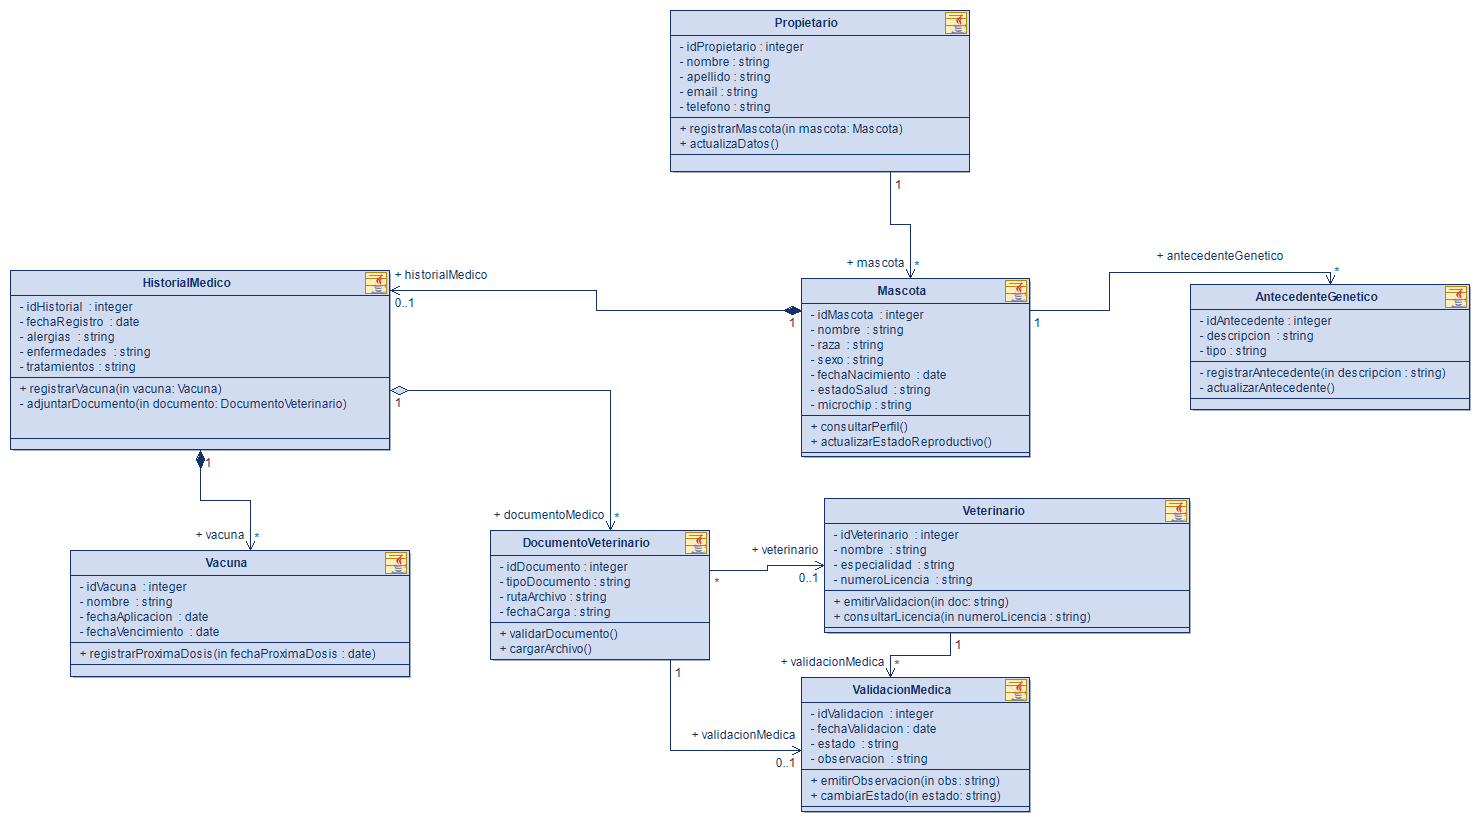
\includegraphics[width=0.82\textwidth]
		{figuras/diagrama_clases.png}
		\caption{Diagrama de clases UML del subsistema MundiPets.}
		\label{fig:diagrama-clases-mundipets}
	\end{figure}
	
	Las responsabilidades principales se resumen en la
	Tabla~\ref{tab:responsabilidades-clases}.
	
	\begin{table}[H]
		\centering
		\caption{Responsabilidades de las clases}
		\label{tab:responsabilidades-clases}
		\footnotesize
		\renewcommand{\arraystretch}{1.02}
		
		\begin{tabularx}{\textwidth}{|p{3.6cm}|Y|}
			\hline
			\textbf{Clase} & \textbf{Responsabilidad} \\
			\hline
			
			\texttt{Propietario} &
			Registrar y administrar las mascotas de su perfil. \\
			\hline
			
			\texttt{Mascota} &
			Centralizar los datos generales y sanitarios del animal. \\
			\hline
			
			\texttt{HistorialMedico} &
			Organizar enfermedades, tratamientos y registros médicos. \\
			\hline
			
			\texttt{Vacuna} &
			Registrar vacunas y sus fechas de aplicación y vencimiento. \\
			\hline
			
			\texttt{DocumentoVeterinario} &
			Representar certificados, informes y archivos médicos. \\
			\hline
			
			\texttt{Veterinario} &
			Consultar información y emitir validaciones profesionales. \\
			\hline
			
			\texttt{ValidacionMedica} &
			Registrar el estado y las observaciones de una validación. \\
			\hline
			
			\texttt{AntecedenteGenetico} &
			Registrar antecedentes y riesgos hereditarios. \\
			\hline
		\end{tabularx}
	\end{table}
	
	\section{Relaciones del modelo}
	
	El diagrama incorpora asociaciones, agregaciones y composiciones. Las
	multiplicidades indican la cantidad de objetos que participan en cada
	relación y permiten que Java Designer genere referencias simples o
	colecciones tipadas.
	
	\begin{itemize}
		\setlength{\itemsep}{2pt}
		\setlength{\parskip}{0pt}
		
		\item \textbf{Propietario--Mascota:}
		asociación uno a muchos. Cada mascota pertenece a un propietario
		(\texttt{1}) y un propietario puede administrar cero o varias
		mascotas (\texttt{0..*}).
		
		\item \textbf{Mascota--HistorialMedico:}
		composición. Una mascota puede tener un historial
		(\texttt{0..1}) y cada historial pertenece a una mascota
		(\texttt{1}).
		
		\item \textbf{Mascota--AntecedenteGenetico:}
		asociación. Una mascota puede registrar varios antecedentes
		(\texttt{0..*}) y cada antecedente pertenece a una mascota
		(\texttt{1}).
		
		\item \textbf{HistorialMedico--Vacuna:}
		composición. Un historial puede contener varias vacunas
		(\texttt{0..*}) y cada vacuna pertenece a un historial
		(\texttt{1}).
		
		\item \textbf{HistorialMedico--DocumentoVeterinario:}
		agregación. Un historial puede reunir varios documentos
		(\texttt{0..*}) y cada documento puede asociarse con un historial
		(\texttt{0..1}).
		
		\item \textbf{Veterinario--DocumentoVeterinario:}
		asociación. Un veterinario puede revisar varios documentos
		(\texttt{0..*}) y cada documento puede relacionarse con un
		veterinario (\texttt{0..1}).
		
		\item \textbf{Veterinario--ValidacionMedica:}
		asociación. Un veterinario puede emitir varias validaciones
		(\texttt{0..*}) y cada validación corresponde a un veterinario
		(\texttt{1}).
		
		\item \textbf{DocumentoVeterinario--ValidacionMedica:}
		asociación. Un documento puede tener una validación
		(\texttt{0..1}) y cada validación se relaciona con un documento
		(\texttt{1}).
		
	\end{itemize}
	
	Las relaciones múltiples pueden transformarse en colecciones como
	\texttt{List<Mascota>}, \texttt{List<Vacuna>} o
	\texttt{List<ValidacionMedica>}. El modelo no incorpora generalización,
	debido a que \texttt{Propietario} y \texttt{Veterinario} se representan
	como clases independientes.
	
	\section{Estereotipo y validación}
	
	Para habilitar la generación se utilizó el perfil de
	\textbf{Java Designer 5.4.00} y se aplicó a las ocho clases el
	estereotipo:
	
	\begin{center}
		\texttt{\textless\textless JavaClass\textgreater\textgreater}
	\end{center}
	
	No se emplearon los estereotipos
	\texttt{\textless\textless Entity\textgreater\textgreater},
	\texttt{\textless\textless Service\textgreater\textgreater} ni
	\texttt{\textless\textless Controller\textgreater\textgreater}, porque
	el generador produce estructuras Java y no implementa automáticamente
	persistencia, servicios o una arquitectura por capas.
	
	La validación se realizó seleccionando el paquete principal y ejecutando:
	
	\begin{center}
		\texttt{Audit $\rightarrow$ Check Model}
	\end{center}
	
	El resultado registró \textbf{cero errores}, \textbf{cero advertencias}
	y \textbf{cero recomendaciones}.
	
	\begin{figure}[H]
		\centering
		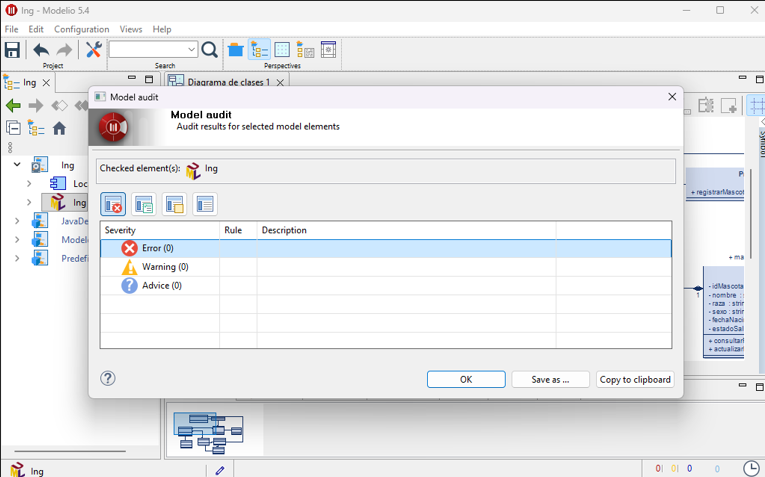
\includegraphics[width=0.58\textwidth]
		{figuras/validacion_modelio.png}
		\caption{Resultado de la auditoría automática del modelo UML.}
		\label{fig:auditoria-modelio}
	\end{figure}
	
	La auditoría se complementó con una revisión manual de tipos, firmas de
	operaciones, multiplicidades, nombres de rol y estereotipos, debido a que
	algunos problemas solo se manifiestan durante la generación o
	compilación del código.
	
	\section{Archivo nativo del modelo}
	
	El proyecto nativo de Modelio, el diagrama UML y las evidencias se
	encuentran almacenados en el repositorio público:
	
	\begin{center}
		\href{
			https://github.com/MoralesGaryUteq/PFC-MundiPets-MDD-EquipoE
		}{
			Repositorio del modelo MundiPets en GitHub
		}
	\end{center}
	
	
	%==================================
	% CAPÍTULO 5
	%==================================
	
	\chapter{CONFIGURACIÓN Y GENERACIÓN DEL CÓDIGO FUENTE}
	
	\section{Configuración del generador}
	
	La transformación del modelo UML hacia código fuente se realizó mediante
	\textbf{Java Designer 5.4.00}, módulo incorporado en
	\textbf{Modelio 5.4.01}, compilación \texttt{202312071609}, para
	arquitectura Windows x86\_64.
	
	Se utilizó el generador estándar proporcionado por Java Designer. Esta
	decisión no respondió a una omisión del proceso de configuración. En la
	instalación utilizada, el módulo no expone desde su interfaz archivos de
	plantilla editables por el usuario. Por tanto, no se efectuó una
	personalización artificial que no pudiera reproducirse posteriormente.
	
	La configuración se controló mediante los elementos que Java Designer
	interpreta directamente desde el modelo: estereotipos, tipos de datos,
	firmas de operaciones, multiplicidades, nombres de rol y visibilidad.
	Para identificar las clases generables se aplicó el estereotipo:
	
	\begin{center}
		\texttt{\textless\textless JavaClass\textgreater\textgreater}
	\end{center}
	
	La configuración utilizada se resume en la
	Tabla~\ref{tab:configuracion-generador}.
	
	\begin{table}[H]
		\centering
		\caption{Configuración del generador Java Designer}
		\label{tab:configuracion-generador}
		\footnotesize
		\renewcommand{\arraystretch}{1.05}
		
		\begin{tabularx}{\textwidth}{|p{4.4cm}|Y|}
			\hline
			\textbf{Parámetro} &
			\textbf{Configuración aplicada} \\
			\hline
			
			Entorno de modelado &
			Modelio 5.4.01. \\
			\hline
			
			Generador &
			Java Designer 5.4.00, generador estándar del módulo. \\
			\hline
			
			Lenguaje objetivo &
			Java. \\
			\hline
			
			Estereotipo de generación &
			\texttt{\textless\textless JavaClass\textgreater\textgreater}. \\
			\hline
			
			Directorio de salida &
			\path{C:/Users/USER/modelio/workspace/Ing/src}. \\
			\hline
			
			Convención de nombres &
			Cada archivo conserva el nombre de su clase UML y utiliza la
			extensión \texttt{.java}. \\
			\hline
			
			Fuente autoritativa &
			El modelo UML construido en Modelio. \\
			\hline
			
			Política de regeneración &
			Los cambios estructurales se corrigen en el modelo y después se
			regenera el archivo correspondiente. \\
			\hline
			
			Código manual &
			Se mantiene separado del código generado; únicamente
			\texttt{Main.java} fue escrito manualmente. \\
			\hline
		\end{tabularx}
	\end{table}
	
	Debido a que no se personalizaron plantillas, se creó el archivo
	\texttt{plantillas/configuracion-java-designer.md} dentro del repositorio.
	Este archivo registra la versión del generador, los parámetros efectivos,
	las convenciones de nombres, las decisiones de mapeo, la política de
	regeneración y las limitaciones observadas. De esta manera, la
	configuración puede ser revisada y reproducida sin atribuir al módulo
	capacidades de edición que no fueron utilizadas.
	
	\section{Procedimiento de generación}
	
	La generación se ejecutó individualmente sobre las clases seleccionadas
	mediante el siguiente procedimiento:
	
	\begin{enumerate}
		
		\item Abrir el proyecto MundiPets en Modelio 5.4.01 y comprobar que
		Java Designer 5.4.00 estuviera habilitado.
		
		\item Verificar la aplicación del estereotipo
		\texttt{\textless\textless JavaClass\textgreater\textgreater}
		en las clases destinadas a generación.
		
		\item Seleccionar cada clase y ejecutar la opción
		\texttt{Java Designer $\rightarrow$ Generate}.
		
		\item Comprobar la creación de los archivos \texttt{.java} en el
		directorio \texttt{src} y revisarlos mediante Visual Studio Code.
		
	\end{enumerate}
	
	Las capturas de la habilitación del módulo, la aplicación del
	estereotipo, la ejecución del generador y los archivos obtenidos se
	presentan en los anexos.
	
	El modelo UML se mantuvo como fuente principal de la estructura del
	código. Los errores relacionados con atributos, tipos, parámetros,
	operaciones, multiplicidades o nombres de rol fueron corregidos
	directamente en Modelio y no únicamente en los archivos Java.
	
	El código escrito manualmente se mantuvo separado del código producido
	por Java Designer. No se evaluó la conservación automática de bloques
	protegidos ni de modificaciones manuales dentro de archivos
	regenerados.
	
	\section{Transformación UML a código Java}
	
	El proceso realizado corresponde a una transformación
	\textbf{Modelo a Texto (M2T)}, debido a que los elementos estructurados
	del modelo UML fueron convertidos en archivos textuales con extensión
	\texttt{.java}.
	
	La correspondencia principal observada se presenta en la
	Tabla~\ref{tab:mapeo-uml-java}.
	
	\begin{table}[H]
		\centering
		\caption{Decisiones de mapeo entre UML y Java}
		\label{tab:mapeo-uml-java}
		\footnotesize
		\renewcommand{\arraystretch}{1.05}
		
		\begin{tabularx}{\textwidth}{|p{4.5cm}|Y|}
			\hline
			\textbf{Elemento UML} &
			\textbf{Decisión de mapeo aplicada} \\
			\hline
			
			Clase con
			\texttt{\textless\textless JavaClass\textgreater\textgreater} &
			Se genera una declaración de clase y un archivo
			\texttt{NombreClase.java}. \\
			\hline
			
			Atributo \texttt{string} &
			Se transforma en un campo Java de tipo \texttt{String}. \\
			\hline
			
			Atributo \texttt{integer} &
			Se transforma en un campo Java de tipo \texttt{int}. \\
			\hline
			
			Atributo \texttt{date} &
			Se transforma en \texttt{Date} con la importación correspondiente. \\
			\hline
			
			Operación UML &
			Se genera un método con nombre, parámetros y tipo de retorno. \\
			\hline
			
			Parámetro de dominio &
			Se utiliza la clase correspondiente, por ejemplo
			\texttt{Mascota mascota},
			\texttt{Vacuna vacuna} o
			\texttt{DocumentoVeterinario documento}. \\
			\hline
			
			Multiplicidad \texttt{0..1} o \texttt{1} &
			Se genera una referencia simple a la clase relacionada. \\
			\hline
			
			Multiplicidad \texttt{0..*} o \texttt{*} &
			Se genera una colección tipada, por ejemplo
			\texttt{List<ValidacionMedica>}. \\
			\hline
			
			Nombre de rol &
			Se utiliza como nombre del campo asociado; los roles múltiples se
			definieron en plural. \\
			\hline
			
			Agregación o composición &
			Se representa estructuralmente mediante referencias o colecciones.
			La gestión del ciclo de vida no es implementada automáticamente. \\
			\hline
		\end{tabularx}
	\end{table}
	
	Java Designer produjo declaraciones de clases, atributos, operaciones,
	referencias y colecciones derivadas de las multiplicidades. El modelo
	actual no incorpora relaciones de generalización; por ello, el código
	generado no utiliza \texttt{extends} entre
	\texttt{Propietario} y \texttt{Veterinario}.
	
	Los cuerpos de varias operaciones permanecieron vacíos, debido a que el
	generador produce principalmente la estructura inicial de las clases.
	La lógica de negocio, persistencia, interfaz gráfica y conexión con bases
	de datos deben implementarse manualmente.
	
	La compilación, ejecución y verificación de los archivos obtenidos se
	documentan en el capítulo siguiente.
	
	
	
	
	%==================================
	% CAPÍTULO 6
	%==================================
	
	\chapter{VERIFICACIÓN DEL SOFTWARE GENERADO}
	
	\section{Proceso de compilación}
	
	La verificación se realizó desde la consola de Windows en el directorio
	donde Java Designer almacenó el código generado
	(\path{C:/Users/USER/modelio/workspace/Ing/src}), confirmando con
	\texttt{javac -version} la disponibilidad de \texttt{javac 17.0.19}.
	Este compilador no intervino en la generación, realizada por Java
	Designer 5.4.00; se utilizó únicamente para verificar la validez
	sintáctica de los archivos obtenidos.
	
	La compilación inicial mediante \texttt{javac *.java} permitió detectar
	parámetros sin nombre, tipos incorrectos y extremos de asociación
	incompletos, incluida una declaración sin nombre de campo
	(\texttt{private Propietario ;}). Las inconsistencias se corrigieron
	directamente en el modelo UML y las clases afectadas fueron
	regeneradas, manteniendo el modelo como fuente principal del código.
	Tras las correcciones, \texttt{javac *.java} no reportó errores y
	produjo ocho archivos compilados: \texttt{AntecedenteGenetico.class},
	\texttt{DocumentoVeterinario.class}, \texttt{HistorialMedico.class},
	\texttt{Mascota.class}, \texttt{Propietario.class}, \texttt{Vacuna.class},
	
	\texttt{ValidacionMedica.class} y \texttt{Veterinario.class}.
	
	\begin{figure}[H]
		\centering
		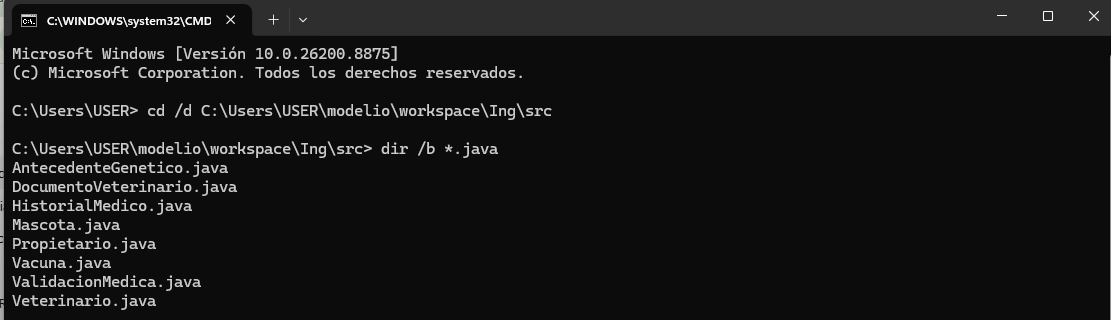
\includegraphics[width=0.80\textwidth]
		{figuras/compilacion_final.png}
		\caption{Compilación exitosa de las ocho clases Java generadas
			mediante Java Designer.}
		\label{fig:compilacion-final}
	\end{figure}
	
	La evidencia confirma la correspondencia entre las ocho clases UML,
	los ocho archivos \texttt{.java} y los ocho archivos
	\texttt{.class} obtenidos.
	
	\section{Ejecución de una unidad demostrable}
	
	Las clases generadas representan la estructura del dominio pero no
	incluyen un método principal, por lo que se creó manualmente la clase
	\texttt{Main.java}, separada del código producido por Java Designer.
	Esta unidad instanció las ocho clases (\texttt{Propietario},
	\texttt{Mascota}, \texttt{HistorialMedico}, \texttt{Vacuna},
	\texttt{DocumentoVeterinario}, \texttt{Veterinario},
	\texttt{ValidacionMedica} y \texttt{AntecedenteGenetico}), confirmó el
	mensaje \texttt{Total de clases verificadas: 8} y terminó con
	\texttt{Process finished with exit code 0}.
	
	\begin{figure}[H]
		\centering
		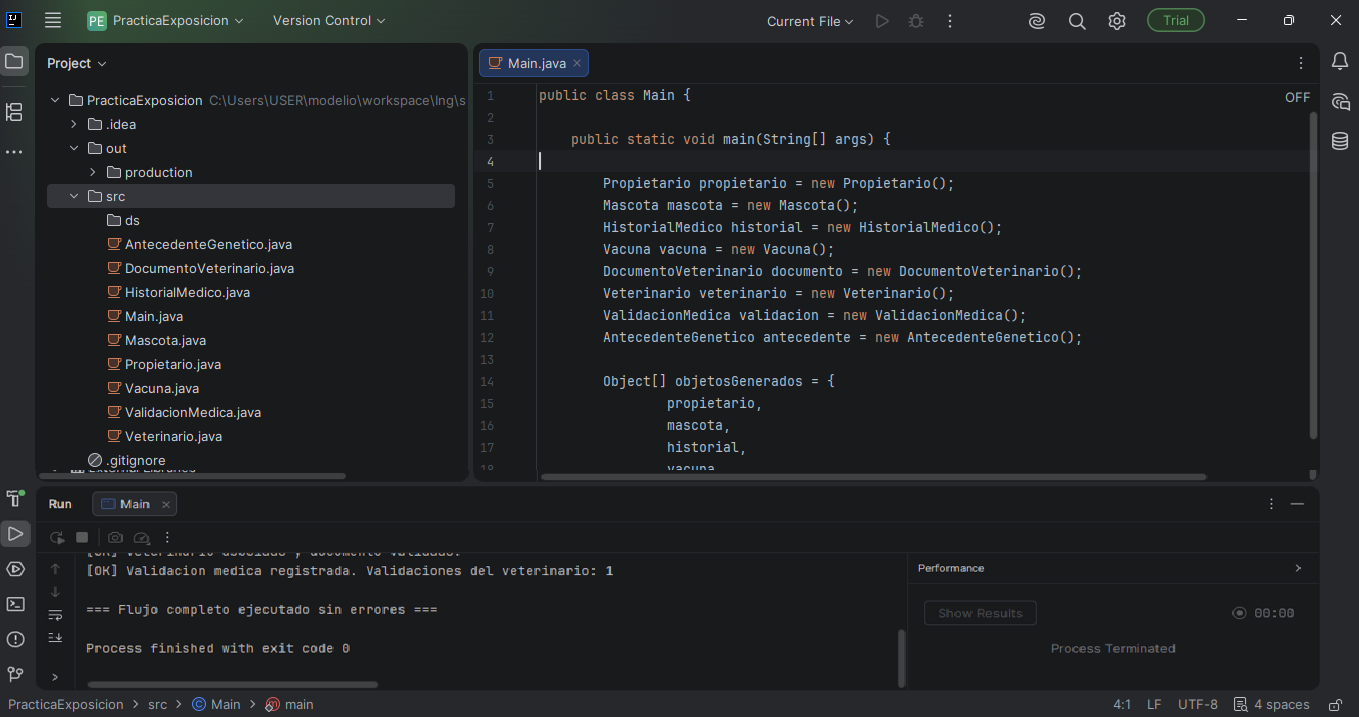
\includegraphics[width=0.80\textwidth]
		{figuras/ejecucion_prueba_mundipets.png}
		\caption{Ejecución de las ocho clases mediante la unidad demostrable
			\texttt{Main.java}.}
		\label{fig:ejecucion-main}
	\end{figure}
	
	La clase \texttt{Main.java} corresponde a código manual y no se
	contabiliza dentro de las ocho clases generadas.
	
	\section{Resultados y correspondencia modelo--código}
	
	La verificación no se limitó a contar los archivos generados. También
	se compararon las clases, atributos, operaciones y asociaciones
	definidos en el modelo UML con las declaraciones producidas por
	Java Designer.
	
	La Tabla~\ref{tab:correspondencia-detallada} presenta la trazabilidad
	entre elementos concretos del modelo y su representación en Java.
	
	\begin{table}[H]
		\centering
		\caption{Correspondencia detallada entre el modelo UML y el código Java}
		\label{tab:correspondencia-detallada}
		\scriptsize
		\renewcommand{\arraystretch}{1.05}
		
		\begin{tabularx}{\textwidth}
			{|p{2.6cm}|p{5.1cm}|Y|}
			\hline
			
			\textbf{Clase / archivo} &
			\textbf{Elemento definido en UML} &
			\textbf{Representación verificada en Java} \\
			\hline
			
			\texttt{Propietario} &
			\texttt{idPropietario:integer};
			operación \texttt{registrarMascota(Mascota)};
			asociación \texttt{mascotas[0..*]} &
			\texttt{private int idPropietario};
			método con parámetro \texttt{Mascota};
			colección \texttt{List<Mascota> mascotas}
			en \texttt{Propietario.java}. \\
			\hline
			
			\texttt{Mascota} &
			\texttt{idMascota:integer},
			\texttt{fechaNacimiento:date} y
			\texttt{microchip:string} &
			Campos \texttt{int idMascota},
			\texttt{Date fechaNacimiento} y
			\texttt{String microchip}
			en \texttt{Mascota.java}. \\
			\hline
			
			\texttt{HistorialMedico} &
			\texttt{fechaRegistro:date};
			operaciones
			\texttt{registrarVacuna(Vacuna)} y
			\texttt{adjuntarDocumento(DocumentoVeterinario)} &
			Campo \texttt{Date fechaRegistro} y métodos con parámetros
			\texttt{Vacuna} y \texttt{DocumentoVeterinario}
			en \texttt{HistorialMedico.java}. \\
			\hline
			
			\texttt{Vacuna} &
			\texttt{idVacuna:integer},
			\texttt{fechaAplicacion:date} y
			\texttt{fechaVencimiento:date} &
			Campos \texttt{int idVacuna},
			\texttt{Date fechaAplicacion} y
			\texttt{Date fechaVencimiento}
			en \texttt{Vacuna.java}. \\
			\hline
			
			\texttt{DocumentoVeterinario} &
			\texttt{idDocumento:integer},
			\texttt{rutaArchivo:string};
			operaciones \texttt{validarDocumento()} y
			\texttt{cargarArchivo()} &
			Campos \texttt{int idDocumento},
			\texttt{String rutaArchivo} y métodos correspondientes
			en \texttt{DocumentoVeterinario.java}. \\
			\hline
			
			\texttt{Veterinario} &
			\texttt{numeroLicencia:string};
			asociación múltiple con
			\texttt{ValidacionMedica} &
			Campo \texttt{String numeroLicencia} y colección
			\texttt{List<ValidacionMedica>}
			en \texttt{Veterinario.java}. \\
			\hline
			
			\texttt{ValidacionMedica} &
			\texttt{idValidacion:integer},
			\texttt{estado:string};
			operaciones \texttt{emitirObservacion(String)} y
			\texttt{cambiarEstado(String)} &
			Campos \texttt{int idValidacion},
			\texttt{String estado} y métodos con parámetros
			\texttt{String}
			en \texttt{ValidacionMedica.java}. \\
			\hline
			
			\texttt{AntecedenteGenetico} &
			\texttt{idAntecedente:integer},
			\texttt{descripcion:string} y
			\texttt{tipo:string} &
			Campos \texttt{int idAntecedente},
			\texttt{String descripcion} y
			\texttt{String tipo}
			en \texttt{AntecedenteGenetico.java}. \\
			\hline
		\end{tabularx}
	\end{table}
	
	La comparación confirmó una correspondencia verificable entre las
	ocho clases del modelo, sus atributos tipados, sus operaciones y los
	ocho archivos Java generados. Las asociaciones con multiplicidad
	múltiple se representaron mediante colecciones tipadas, mientras que
	las multiplicidades máximas de uno produjeron referencias simples.
	
	\section{Limitaciones encontradas}
	
	\begin{itemize}
		\setlength{\itemsep}{1pt}
		
		\item Java Designer genera principalmente la estructura de las clases,
		pero no implementa completamente la lógica de negocio.
		
		\item La ejecución requiere una clase principal escrita manualmente.
		
		\item La persistencia, la interfaz gráfica y la conexión con bases de
		datos deben incorporarse posteriormente.
		
		\item La auditoría automática debe complementarse con revisión manual,
		compilación y ejecución del código.
		
	\end{itemize}
	
	En consecuencia, Java Designer facilita la trazabilidad estructural
	entre UML y Java, pero no sustituye la implementación manual necesaria
	para obtener una aplicación completamente funcional.
	
	
	
	%==================================
	% CAPÍTULO 7
	%==================================
	
	\chapter{ROUNDTRIP ENGINEERING}
	
	\section{Modificación controlada del modelo UML}
	
	Para comprobar el cierre controlado del ciclo modelo--código, se
	incorporó a la clase \texttt{Mascota} el atributo
	\texttt{microchip : string} y la operación
	\texttt{actualizarMicrochip(in nuevoMicrochip:string):void}, que
	permiten almacenar y actualizar el identificador electrónico de la
	mascota. Antes del cambio, la clase contenía únicamente los atributos
	\texttt{idMascota}, \texttt{nombre}, \texttt{raza}, \texttt{sexo},
	\texttt{fechaNacimiento} y \texttt{estadoSalud}, y las operaciones
	\texttt{consultarPerfil()} y \texttt{actualizarEstadoReproductivo()}.
	
	\begin{figure}[H]
		\centering
		
		\begin{minipage}{0.48\textwidth}
			\centering
			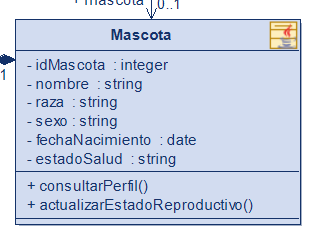
\includegraphics[width=\linewidth]
			{figuras/roundtrip_modelo_antes.png}
			
			\small (a) Clase \texttt{Mascota} antes del cambio.
		\end{minipage}
		\hfill
		\begin{minipage}{0.48\textwidth}
			\centering
			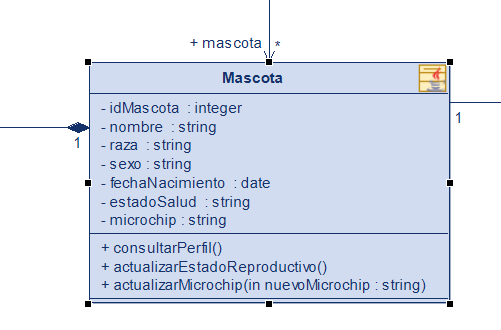
\includegraphics[width=\linewidth]
			{figuras/roundtrip_modelo_despues.png}
			
			\small (b) Clase \texttt{Mascota} después del cambio.
		\end{minipage}
		
		\caption{Modelo UML antes y después de incorporar el atributo
			\texttt{microchip} y la operación
			\texttt{actualizarMicrochip}.}
		\label{fig:roundtrip-modelo}
	\end{figure}
	
	La modificación se considera un cambio estructural compuesto porque
	afecta simultáneamente un atributo, una operación, un parámetro, un tipo
	de retorno y la estructura del archivo Java generado. Los elementos se
	incorporaron directamente en Modelio, manteniendo el modelo UML como
	fuente principal del código.
	
	\section{Regeneración del código fuente}
	
	Después de modificar la clase \texttt{Mascota}, se ejecutó nuevamente
	\texttt{Java Designer $\rightarrow$ Generate} sobre el archivo
	\texttt{Mascota.java} almacenado en
	\path{C:/Users/USER/modelio/workspace/Ing/src}. El atributo UML se
	transformó en el campo \texttt{private String microchip;} y la
	operación se transformó en el método:
	
	\begin{verbatim}
		public void actualizarMicrochip(
		final String nuevoMicrochip) {
		}
	\end{verbatim}
	
	El cuerpo del método permaneció vacío porque Java Designer genera
	principalmente la estructura de las operaciones; ni el campo ni la
	firma fueron escritos manualmente. Tras la regeneración, el código se
	compiló nuevamente mediante \texttt{javac *.java} sin errores,
	confirmando que el nuevo atributo, operación y parámetro fueron
	transformados en estructuras Java sintácticamente válidas.
	
	\section{Comparación antes y después}
	
	La comparación de \texttt{Mascota.java} confirma que los cambios del
	modelo UML se trasladaron al código fuente sin intervención manual.
	
	\begin{figure}[H]
		\centering
		
		\begin{minipage}{0.48\textwidth}
			\centering
			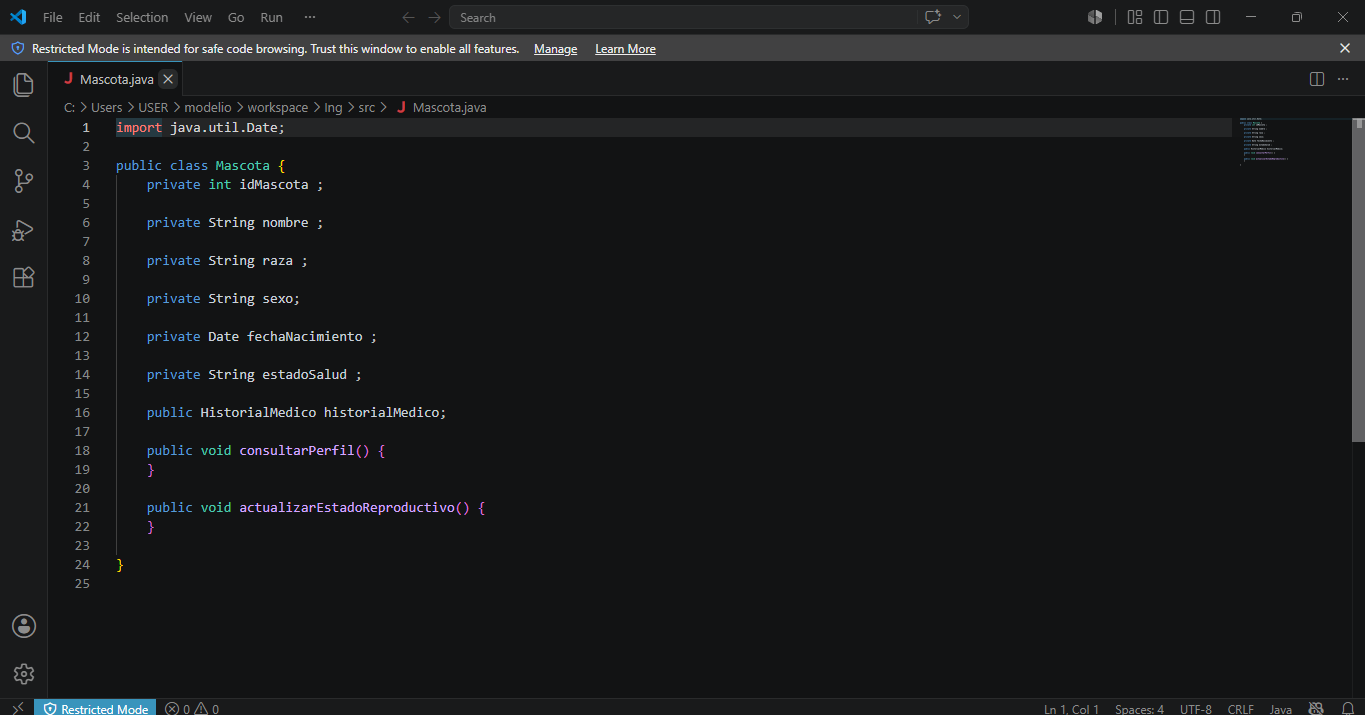
\includegraphics[width=\linewidth]
			{figuras/roundtrip_codigo_antes.png}
			
			\small (a) Código antes de la regeneración.
		\end{minipage}
		\hfill
		\begin{minipage}{0.48\textwidth}
			\centering
			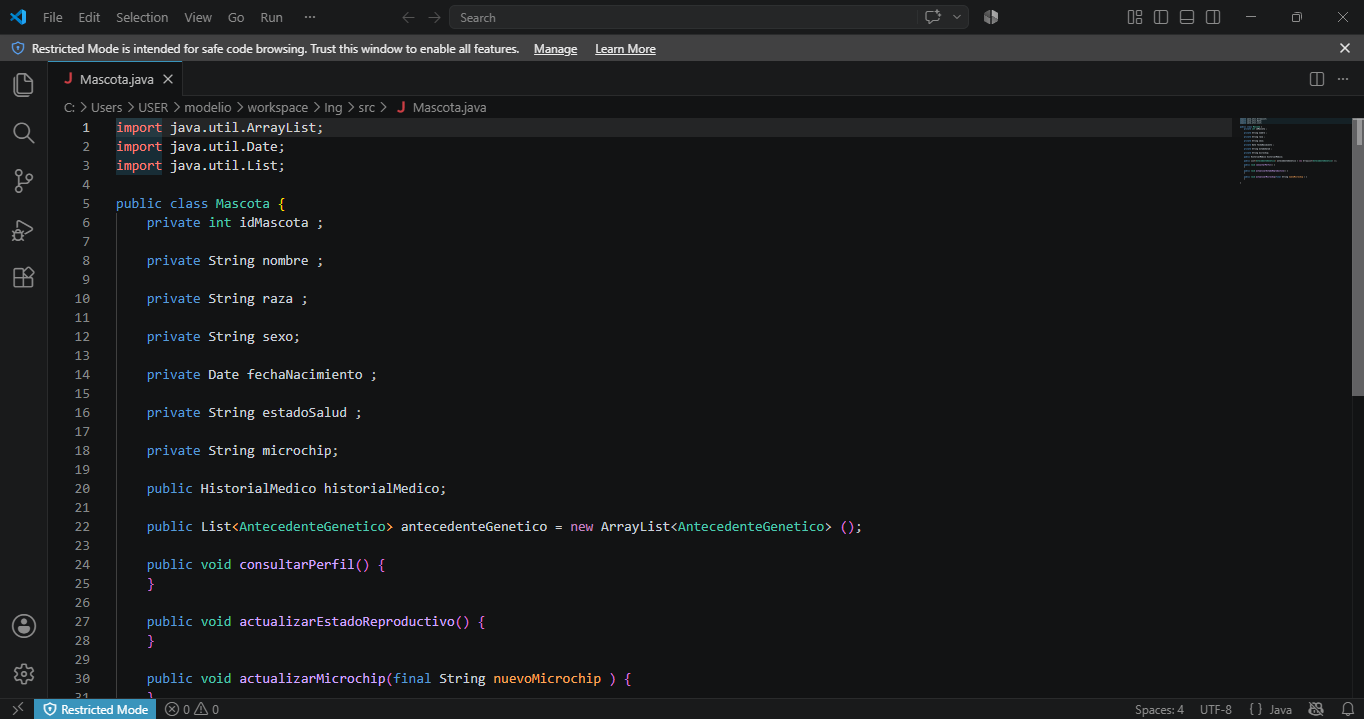
\includegraphics[width=\linewidth]
			{figuras/roundtrip_codigo_despues.png}
			
			\small (b) Código después de la regeneración.
		\end{minipage}
		
		\caption{Código de \texttt{Mascota.java} antes y después de generar
			el atributo y la operación incorporados en el modelo UML.}
		\label{fig:roundtrip-codigo}
	\end{figure}
	
	La Tabla~\ref{tab:comparacion-roundtrip} presenta la trazabilidad del
	cambio realizado.
	
	\begin{table}[H]
		\centering
		\caption{Comparación del cambio realizado durante el roundtrip}
		\label{tab:comparacion-roundtrip}
		\footnotesize
		\renewcommand{\arraystretch}{1.05}
		
		\begin{tabularx}{\textwidth}{|p{3.2cm}|Y|Y|}
			\hline
			\textbf{Elemento} &
			\textbf{Antes del cambio} &
			\textbf{Después del cambio} \\
			\hline
			
			Atributo UML &
			No existía el atributo
			\texttt{microchip}. &
			Se incorporó
			\texttt{microchip:string}. \\
			\hline
			
			Operación UML &
			No existía una operación para actualizar el identificador. &
			Se incorporó
			\texttt{actualizarMicrochip(in nuevoMicrochip:string):void}. \\
			\hline
			
			Campo Java &
			No existía un campo para almacenar el microchip. &
			Se generó
			\texttt{private String microchip;}. \\
			\hline
			
			Método Java &
			No existía un método de actualización. &
			Se generó
			\texttt{actualizarMicrochip(String nuevoMicrochip)}. \\
			\hline
			
			Parámetro &
			No existía un parámetro relacionado con el microchip. &
			Se generó el parámetro
			\texttt{final String nuevoMicrochip}. \\
			\hline
			
			Intervención manual &
			No se modificó directamente el archivo generado. &
			El cambio se realizó en Modelio y se regeneró
			\texttt{Mascota.java}. \\
			\hline
			
			Compilación &
			El código anterior compilaba correctamente. &
			El código regenerado volvió a compilar sin errores. \\
			\hline
		\end{tabularx}
	\end{table}
	
	La evidencia demuestra la trazabilidad
	\textbf{atributo y operación UML $\rightarrow$ campo, método y
		parámetro Java}: un cierre controlado del ciclo modelo--código, en el
	que la modificación se realizó en Modelio y los nuevos elementos
	aparecieron en \texttt{Mascota.java} sin ser incorporados manualmente.
	
	\section{Manejo del código manual}
	
	La evidencia presentada no constituye una sincronización bidireccional
	completa, ya que el código Java no fue modificado para actualizar
	posteriormente el modelo UML. En la configuración estándar de Java
	Designer 5.4.00 no se comprobó la conservación automática de bloques
	protegidos, por lo que las ocho clases producidas se trataron como
	archivos generados y reemplazables. La clase \texttt{Main.java} y
	cualquier lógica manual se mantuvieron separadas del código generado,
	evitando que una regeneración sobrescriba la implementación manual.
	
	
	
	%==================================
	% CAPÍTULO 8
	%==================================
	
	\chapter{REPOSITORIO GITHUB Y TRABAJO COLABORATIVO}
	
	\section{Organización del repositorio}
	
	Los artefactos desarrollados durante la aplicación del enfoque MDD se
	almacenaron en un repositorio público de GitHub. Este recurso permitió
	centralizar el modelo UML, el código generado, el informe en LaTeX y las
	evidencias de generación, compilación, ejecución y roundtrip.
	
	El repositorio se encuentra disponible en:
	
	\begin{center}
		\href{
			https://github.com/MoralesGaryUteq/PFC-MundiPets-MDD-EquipoE
		}{
			\texttt{PFC--MundiPets--MDD--EquipoE}
		}
	\end{center}
	
	La estructura principal del repositorio se resume en la
	Tabla~\ref{tab:estructura-repositorio}.
	
	\begin{table}[H]
		\centering
		\caption{Estructura principal del repositorio}
		\label{tab:estructura-repositorio}
		\small
		\renewcommand{\arraystretch}{1.10}
		
		\begin{tabularx}{\textwidth}{|p{4cm}|Y|}
			\hline
			\textbf{Elemento} & \textbf{Contenido} \\
			\hline
			
			\texttt{README.md} &
			Descripción, integrantes, herramientas e instrucciones generales. \\
			\hline
			
			\texttt{modelo/} &
			Proyecto nativo de Modelio y diagrama UML. \\
			\hline
			
			\texttt{plantillas/} &
			Archivo \texttt{README.md} que documenta la configuración efectiva del generador (módulo Java Designer 5.4.00), justificando por qué no existen plantillas de texto editables al tratarse de un módulo compilado, e indicando el entorno base, fuente oficial y licencia del módulo utilizado. \\
			\hline
			
			\texttt{codigo-generado/} &
			Archivos Java producidos mediante Java Designer. \\
			\hline
			
			\texttt{documentacion/} &
			Informe en LaTeX, bibliografía y PDF final. \\
			\hline
			
			\texttt{evidencias/} &
			Capturas de auditoría, generación, compilación y roundtrip. \\
			\hline
		\end{tabularx}
	\end{table}
	
	\section{Reparto del trabajo por integrante}
	
	
	\textbf{Nota:} esta sección se encuentra pendiente de completar con
	el historial real de commits del repositorio antes de la entrega
	final. La rúbrica exige, para cada integrante, tareas concretas y
	una lista de commits atribuibles con su URL en GitHub; no debe
	entregarse en blanco ni con datos supuestos.
	
	\begin{table}[H]
		\centering
		\caption{Reparto del trabajo por integrante \textit{(pendiente de completar con datos reales)}}
		\label{tab:responsabilidades-equipo}
		\small
		\renewcommand{\arraystretch}{1.15}
		
		\begin{tabularx}{\textwidth}{|p{3.4cm}|p{4.6cm}|Y|}
			\hline
			\textbf{Integrante} &
			\textbf{Fases lideradas / tareas concretas} &
			\textbf{Commits atribuibles (URL)} \\
			\hline
			
			Gary Alejandro Morales Sánchez &
			\textit{Completar modelado UML, verificación de código,  roundtrip.} &
			\textit{[Completar con URLs de commits, ej.:
				github.com/.../commit/abcd123]} \\
			\hline
			
			Jimmy Samuel Nieves Sánchez &
			\textit{Completar onfiguración de Java Designer, marco teórico, generación, compilación, documentación.} &
			\textit{[Completar con URLs de commits]} \\
			\hline
		\end{tabularx}
	\end{table}
	
	Los productos principales fueron revisados de manera conjunta antes de
	su incorporación al repositorio y al documento final.
	
	\section{Evidencias de colaboración}
	
	La participación del equipo se demuestra mediante el historial de
	commits, los archivos modificados y la sección de colaboradores de
	GitHub. Las capturas de la estructura del repositorio, los commits y las
	contribuciones individuales se presentan en los anexos.
	
	
	%==================================
	% CAPÍTULO 9
	%==================================
	
	\chapter{CONCLUSIONES}
	
	\begin{enumerate}
		
		\item La aplicación del enfoque de Desarrollo Dirigido por Modelos
		permitió utilizar el diagrama de clases UML de MundiPets como
		artefacto principal para obtener estructuras de código Java. Esto
		estableció una relación verificable entre el diseño del subsistema y
		los archivos generados.
		
		\item Modelio 5.4.01, mediante el módulo Java Designer 5.4.00,
		permitió transformar las clases, atributos, operaciones,
		asociaciones y relaciones de generalización del modelo UML en
		elementos equivalentes del lenguaje Java. Para realizar esta
		transformación se utilizó el estereotipo
		\texttt{\textless\textless JavaClass\textgreater\textgreater}.
		
		\item La auditoría automática de Modelio no reportó errores,
		advertencias ni recomendaciones. Sin embargo, la compilación permitió
		identificar problemas que no fueron detectados por la validación
		automática, como parámetros sin nombre y extremos de asociaciones
		incompletos. Esto evidencia la necesidad de complementar la auditoría
		del modelo con una revisión manual y con la compilación del código.
		
		\item Después de corregir las definiciones del modelo UML y regenerar
		las clases, la compilación mediante \texttt{javac *.java} terminó sin
		errores y produjo ocho archivos \texttt{.class}. Este resultado
		confirmó que el código estructural generado era válido para el
		compilador de Java.
		
		\item La calidad del código producido depende directamente de la
		precisión del modelo de origen. Los tipos de datos, nombres de
		parámetros, multiplicidades y nombres de rol deben definirse
		correctamente en UML, debido a que cualquier inconsistencia puede
		trasladarse al archivo Java generado.
		
		\item Java Designer facilita la automatización de la estructura
		inicial del software, pero no genera una aplicación completamente
		funcional. La lógica de negocio, persistencia, interfaz de usuario,
		conexión con bases de datos y ejecución mediante un método
		\texttt{main} requieren implementación manual posterior.
		
		\item El uso del repositorio GitHub permitió organizar el modelo
		nativo, el código generado, el informe y las evidencias del proceso,
		proporcionando trazabilidad sobre las actividades desarrolladas y los
		aportes realizados por los integrantes del equipo.
		
	\end{enumerate}
	
	En conclusión, el proyecto demostró que el enfoque MDD permite reducir
	la codificación repetitiva y mantener correspondencia entre el modelo
	UML y el código Java. No obstante, la generación automática debe
	acompañarse de validación, compilación y revisión técnica para garantizar
	que los artefactos obtenidos sean consistentes y utilizables.
	
	
	
	%==================================
	% CAPÍTULO 10
	%==================================
	
	\chapter{REFERENCIAS}
	
	\printbibliography[heading=none]
	
	%==================================
	% CAPÍTULO 11
	%==================================
	
	\chapter{ANEXOS}
	
	Los anexos reúnen las evidencias complementarias del proceso de
	modelado, generación, compilación, regeneración y trabajo colaborativo.
	Estos elementos respaldan los resultados presentados en los capítulos
	anteriores.
	
	%==================================
	% ANEXO: MODELO UML
	%==================================
	
	\section{Diagrama UML completo}
	
	La Figura~\ref{fig:anexo-diagrama-completo} presenta el diagrama de
	clases completo del subsistema de gestión de información de mascotas y
	control veterinario de MundiPets.
	
	\begin{figure}[H]
		\centering
		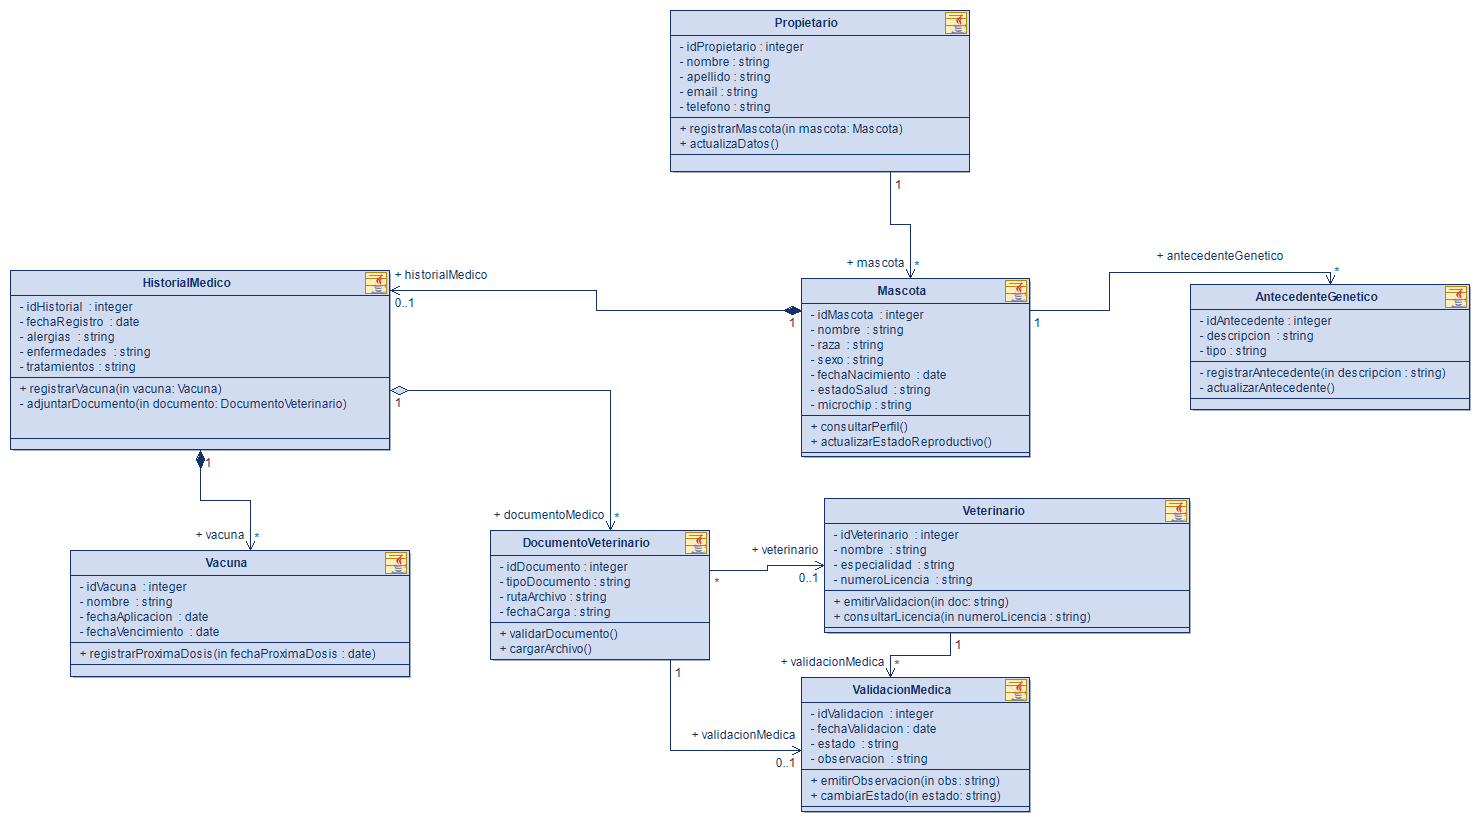
\includegraphics[width=\textwidth]
		{figuras/diagrama_clases.png}
		\caption{Diagrama de clases UML completo del subsistema MundiPets.}
		\label{fig:anexo-diagrama-completo}
	\end{figure}
	
	El archivo nativo del modelo desarrollado en Modelio se encuentra
	almacenado en el repositorio público del proyecto.
	
	%==================================
	% ANEXO: CAPTURAS DE MODELIO
	%==================================
	
	\section{Capturas de la herramienta MDD}
	
	\subsection{Configuración de Java Designer}
	
	\begin{figure}[H]
		\centering
		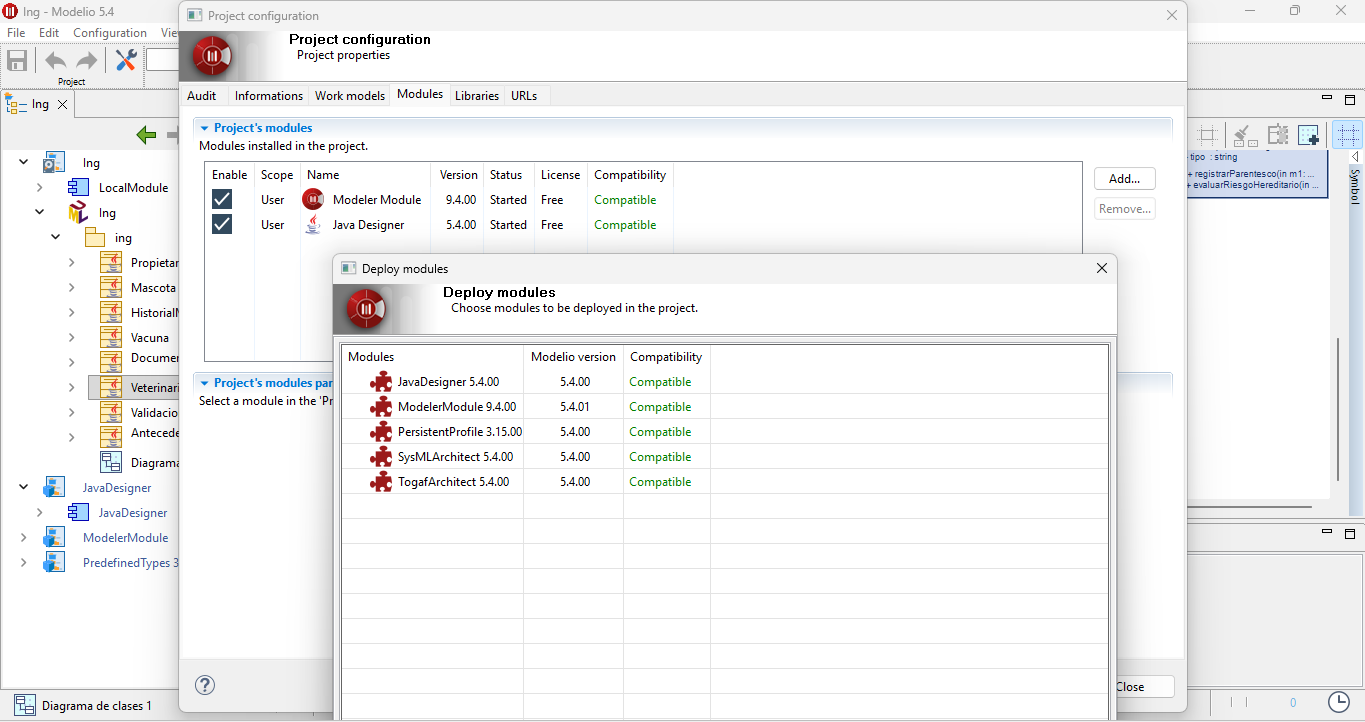
\includegraphics[width=0.90\textwidth]
		{figuras/modulo_java_designer.png}
		\caption{Módulo Java Designer 5.4.00 habilitado en Modelio 5.4.01.}
		\label{fig:anexo-java-designer}
	\end{figure}
	
	\subsection{Aplicación del estereotipo JavaClass}
	
	\begin{figure}[H]
		\centering
		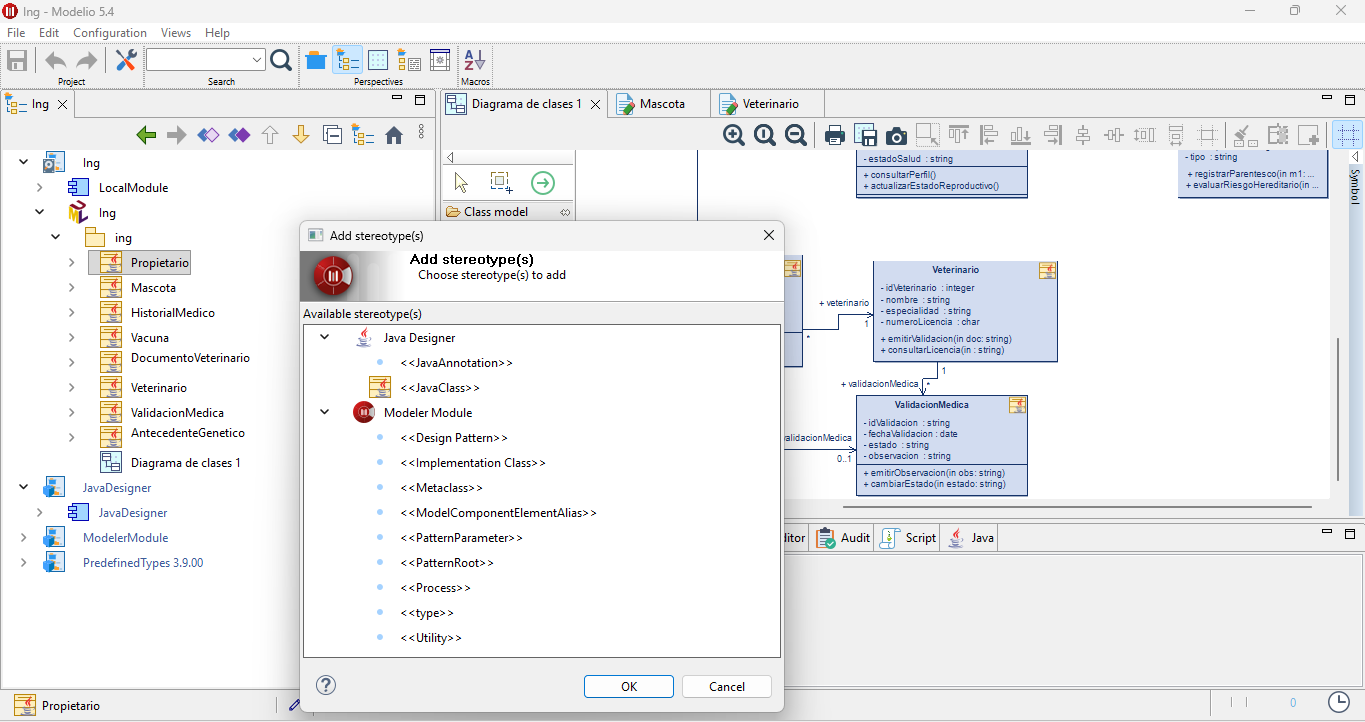
\includegraphics[width=0.88\textwidth]
		{figuras/estereotipo_java_class.png}
		\caption{Aplicación del estereotipo
			\texttt{\textless\textless JavaClass\textgreater\textgreater}
			a una clase UML.}
		\label{fig:anexo-estereotipo}
	\end{figure}
	
	\subsection{Validación automática del modelo}
	
	\begin{figure}[H]
		\centering
		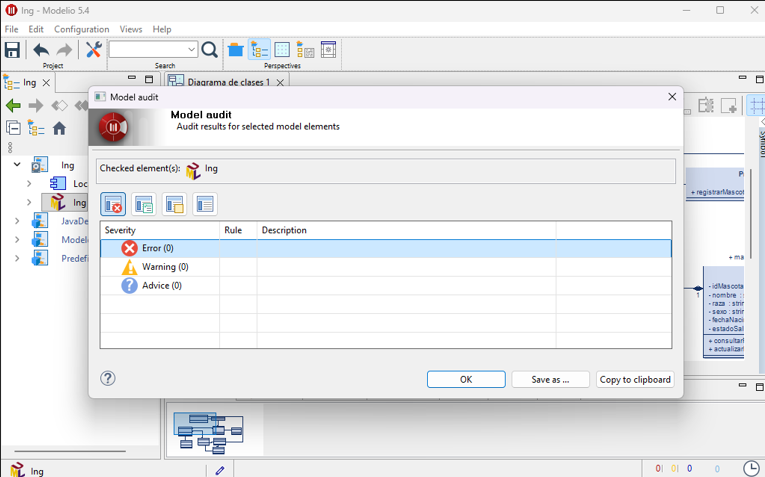
\includegraphics[width=0.88\textwidth]
		{figuras/validacion_modelio.png}
		\caption{Resultado de la auditoría automática ejecutada en Modelio.}
		\label{fig:anexo-validacion-modelio}
	\end{figure}
	
	\subsection{Ejecución del mecanismo de generación}
	
	\begin{figure}[H]
		\centering
		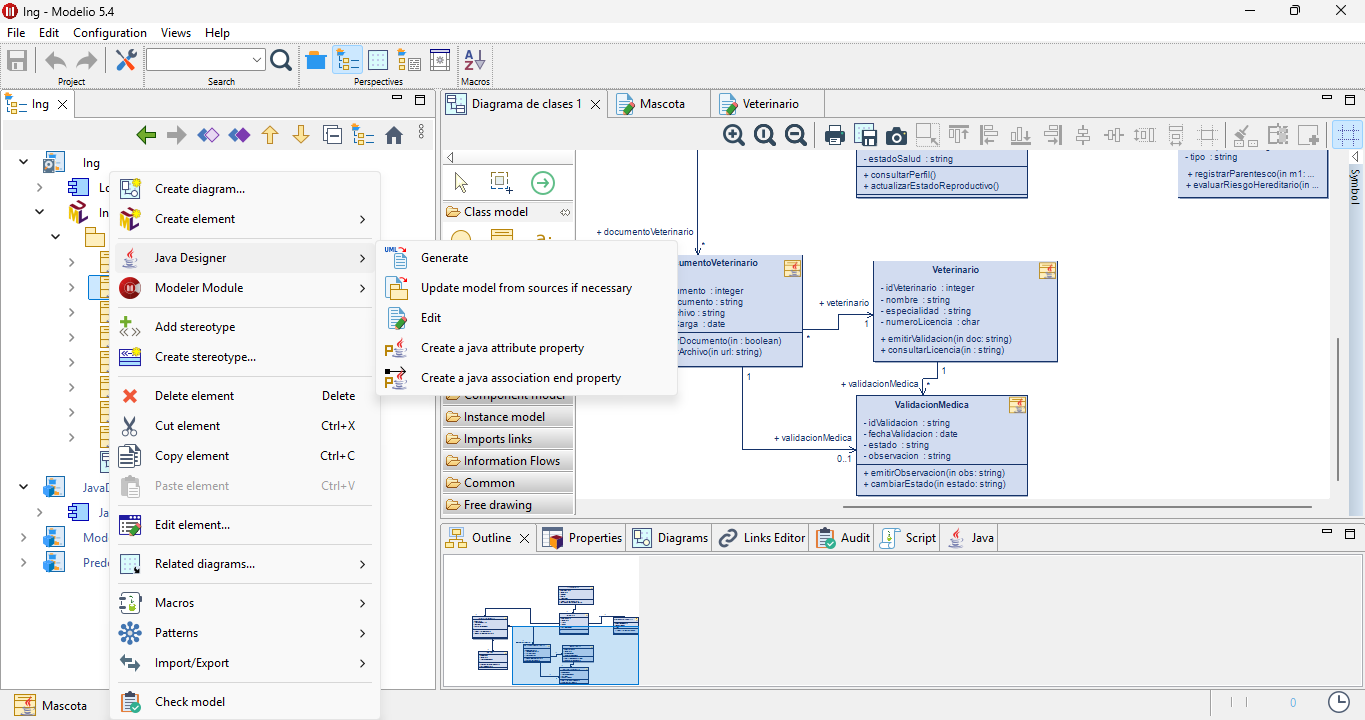
\includegraphics[width=0.88\textwidth]
		{figuras/opcion_generar_codigo.png}
		\caption{Ejecución de la opción Java Designer
			\texorpdfstring{$\rightarrow$}{->} Generate.}
		\label{fig:anexo-generacion}
	\end{figure}
	
	\subsection{Archivos Java generados}
	
	\begin{figure}[H]
		\centering
		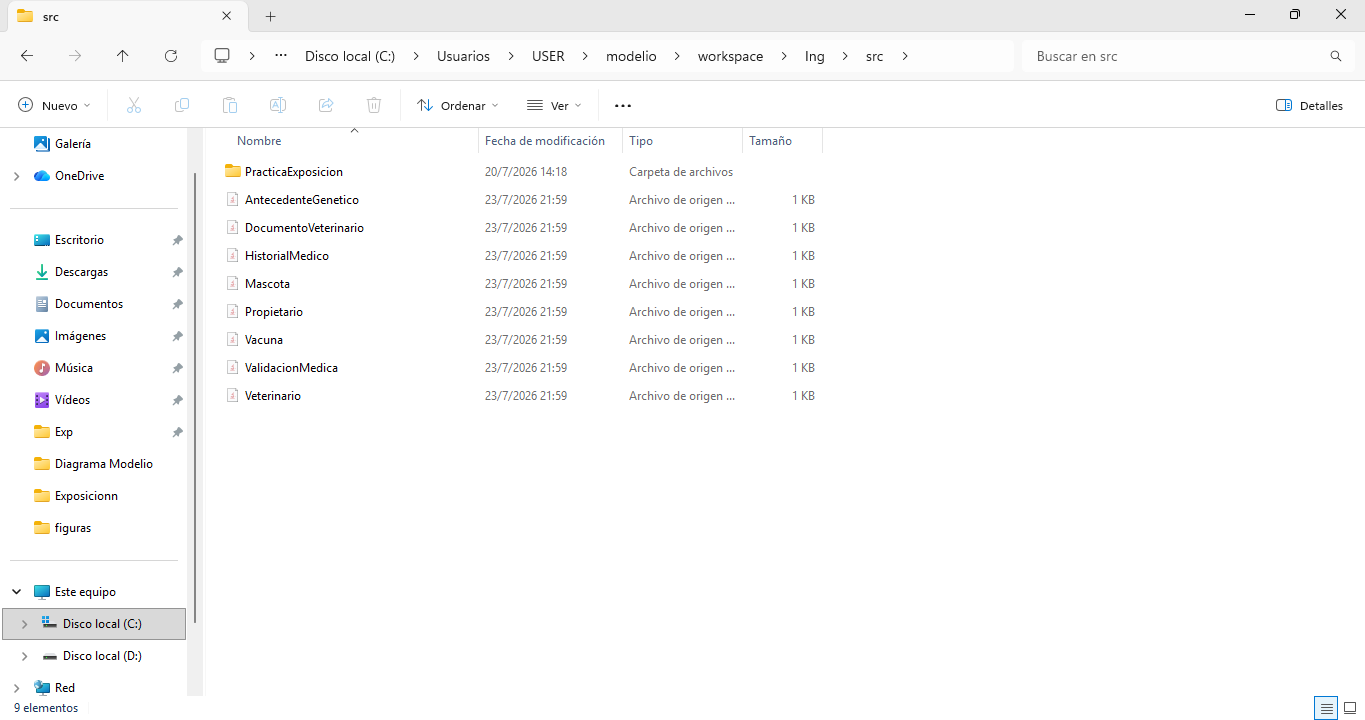
\includegraphics[width=0.92\textwidth]
		{figuras/archivos_java_generados.png}
		\caption{Archivos Java producidos por Java Designer en el directorio
			\texttt{src}.}
		\label{fig:anexo-archivos-generados}
	\end{figure}
	
	%==================================
	% ANEXO: CÓDIGO GENERADO
	%==================================
	
	\section{Código fuente generado}
	
	Los siguientes listados presentan clases representativas obtenidas
	mediante Java Designer. El conjunto completo de archivos se encuentra
	disponible en el repositorio del proyecto.
	
	\Needspace{0.60\textheight}
	
	\subsection{Clase Mascota}
	
	\begin{samepage}
		
		\lstinputlisting[
		language=Java,
		basicstyle=\ttfamily\footnotesize,
		numbers=left,
		numberstyle=\tiny,
		numbersep=6pt,
		frame=single,
		breaklines=true,
		breakatwhitespace=true,
		columns=fullflexible,
		keepspaces=true,
		showstringspaces=false,
		captionpos=b,
		caption={Código generado de la clase Mascota.},
		label={lst:mascota-generada}
		]{codigo-generado/Mascota.txt}
		
	\end{samepage}
	
	\Needspace{0.60\textheight}
	
	\subsection{Clase Propietario}
	
	\begin{samepage}
		
		\lstinputlisting[
		language=Java,
		basicstyle=\ttfamily\footnotesize,
		numbers=left,
		numberstyle=\tiny,
		numbersep=6pt,
		frame=single,
		breaklines=true,
		breakatwhitespace=true,
		columns=fullflexible,
		keepspaces=true,
		showstringspaces=false,
		captionpos=b,
		caption={Código generado de la clase Propietario.},
		label={lst:propietario-generado}
		]{codigo-generado/Propietario.txt}
		
	\end{samepage}
	
	\Needspace{0.60\textheight}
	
	\subsection{Clase Veterinario}
	
	\begin{samepage}
		
		\lstinputlisting[
		language=Java,
		basicstyle=\ttfamily\footnotesize,
		numbers=left,
		numberstyle=\tiny,
		numbersep=6pt,
		frame=single,
		breaklines=true,
		breakatwhitespace=true,
		columns=fullflexible,
		keepspaces=true,
		showstringspaces=false,
		captionpos=b,
		caption={Código generado de la clase Veterinario.},
		label={lst:veterinario-generado}
		]{codigo-generado/Veterinario.txt}
		
	\end{samepage}
	
	%==================================
	% ANEXO: COMPILACIÓN Y EJECUCIÓN
	%==================================
	
	\section{Evidencias de compilación y ejecución}
	
	\subsection{Compilación del código generado}
	
	La compilación se realizó desde la consola de Windows mediante los
	comandos:
	
	\begin{center}
		\texttt{javac *.java}
	\end{center}
	
	\begin{center}
		\texttt{dir *.class}
	\end{center}
	
	\begin{figure}[H]
		\centering
		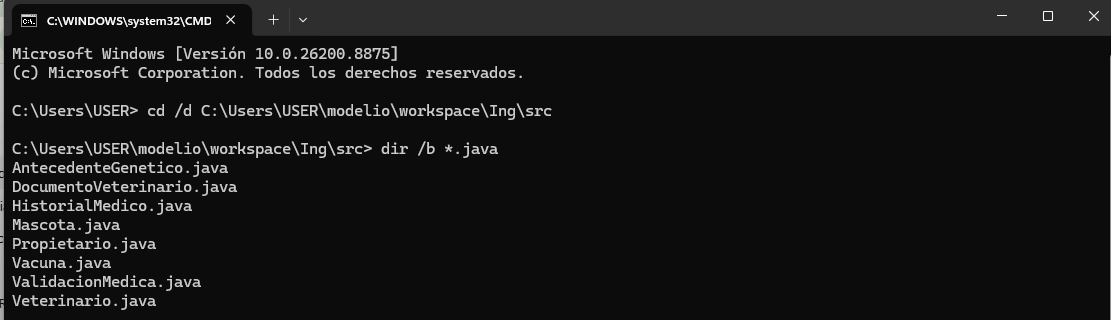
\includegraphics[width=0.94\textwidth]
		{figuras/compilacion_final.png}
		\caption{Compilación exitosa de las clases Java generadas.}
		\label{fig:anexo-compilacion}
	\end{figure}
	
	La consola no reportó errores y mostró ocho archivos
	\texttt{.class}, correspondientes a las clases compiladas.
	
	\subsection{Ejecución de la unidad demostrable}
	
	% Mantener este apartado únicamente cuando se haya ejecutado
	% realmente la clase PruebaMundiPets.
	
	\begin{figure}[H]
		\centering
		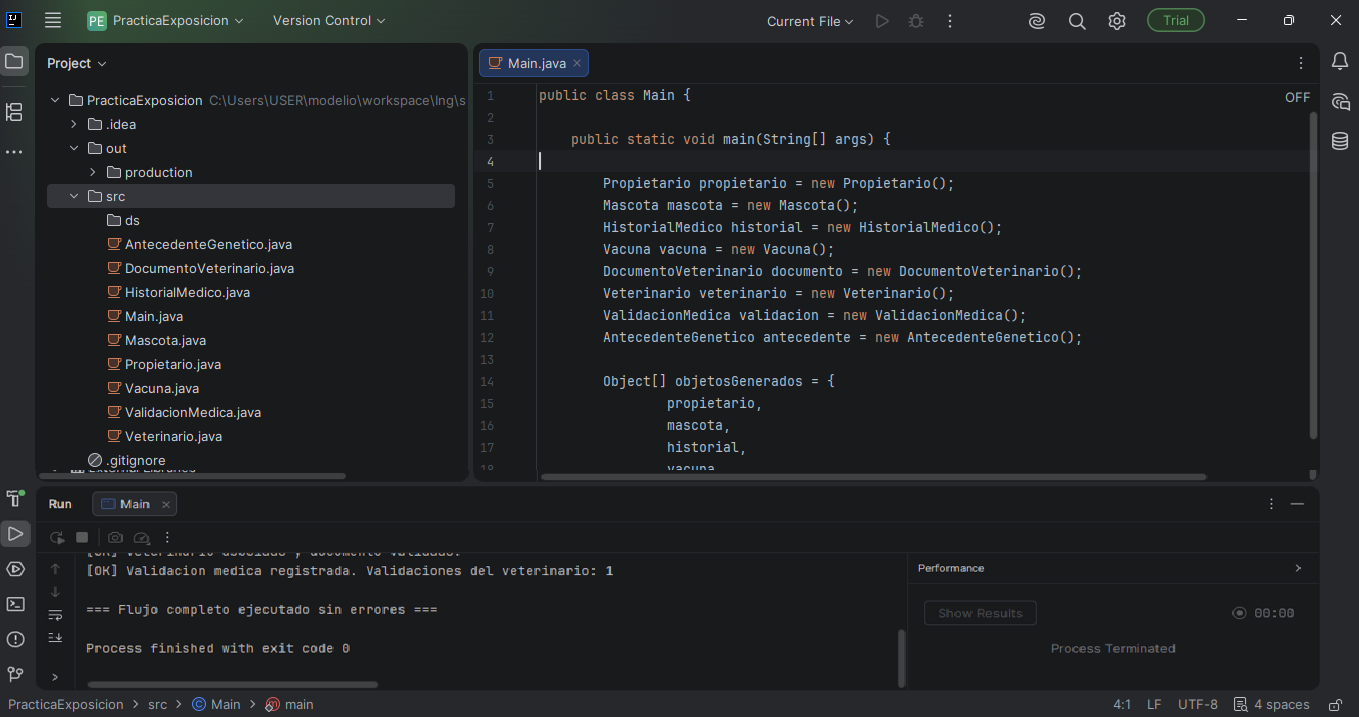
\includegraphics[width=0.94\textwidth]
		{figuras/ejecucion_prueba_mundipets.png}
		\caption{Ejecución de la unidad demostrable
			\texttt{PruebaMundiPets}.}
		\label{fig:anexo-ejecucion}
	\end{figure}
	
	%==================================
	% ANEXO: ROUNDTRIP
	%==================================
	
	\section{Evidencias del roundtrip}
	
	\subsection{Modelo antes y después del cambio}
	
	\begin{figure}[H]
		\centering
		
		\begin{minipage}{0.48\textwidth}
			\centering
			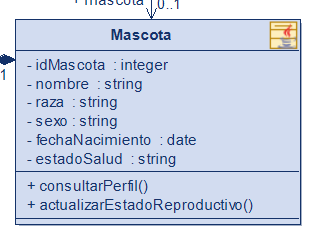
\includegraphics[width=\linewidth]
			{figuras/roundtrip_modelo_antes.png}
			
			\small (a) Modelo antes de la modificación.
		\end{minipage}
		\hfill
		\begin{minipage}{0.48\textwidth}
			\centering
			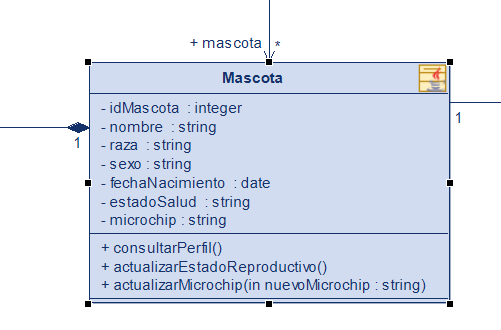
\includegraphics[width=\linewidth]
			{figuras/roundtrip_modelo_despues.png}
			
			\small (b) Modelo después de la modificación.
		\end{minipage}
		
		\caption{Comparación del modelo UML antes y después del cambio
			controlado.}
		\label{fig:anexo-roundtrip-modelo}
	\end{figure}
	
	\subsection{Código antes y después de la regeneración}
	
	\begin{figure}[H]
		\centering
		
		\begin{minipage}{0.48\textwidth}
			\centering
			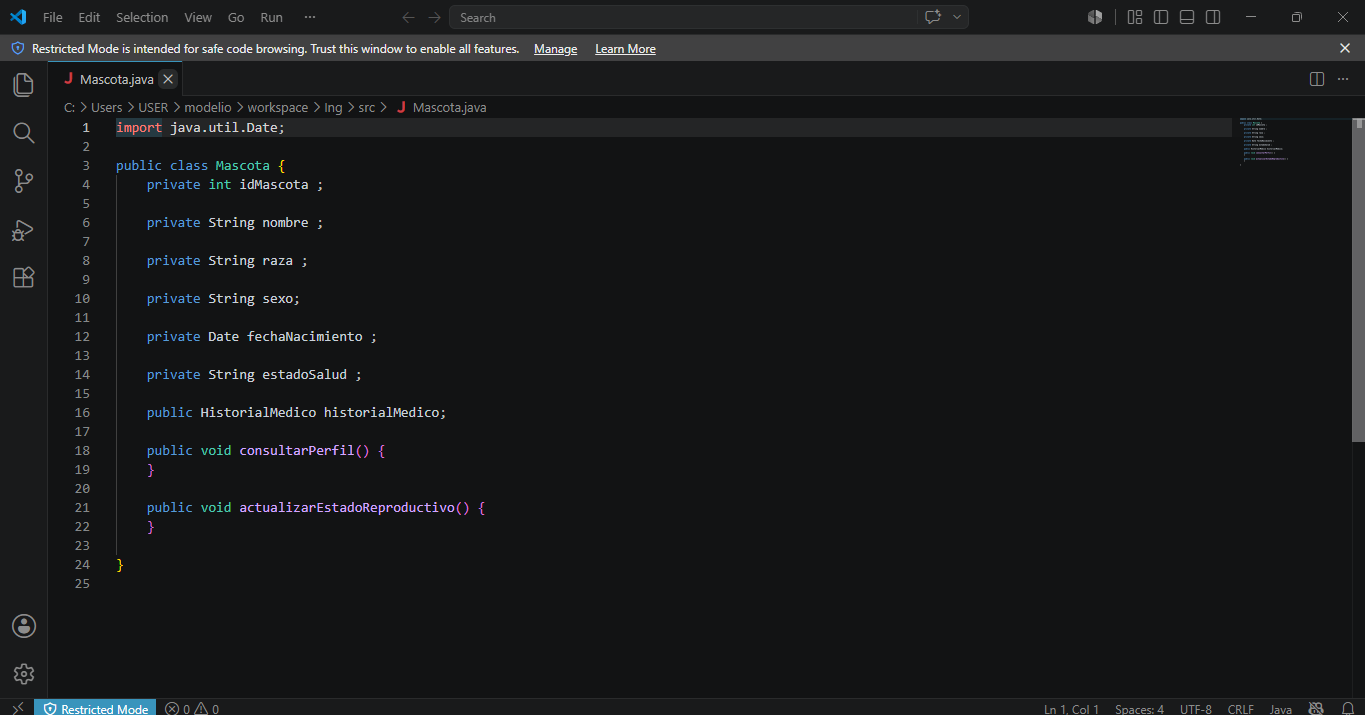
\includegraphics[width=\linewidth]
			{figuras/roundtrip_codigo_antes.png}
			
			\small (a) Código antes de la regeneración.
		\end{minipage}
		\hfill
		\begin{minipage}{0.48\textwidth}
			\centering
			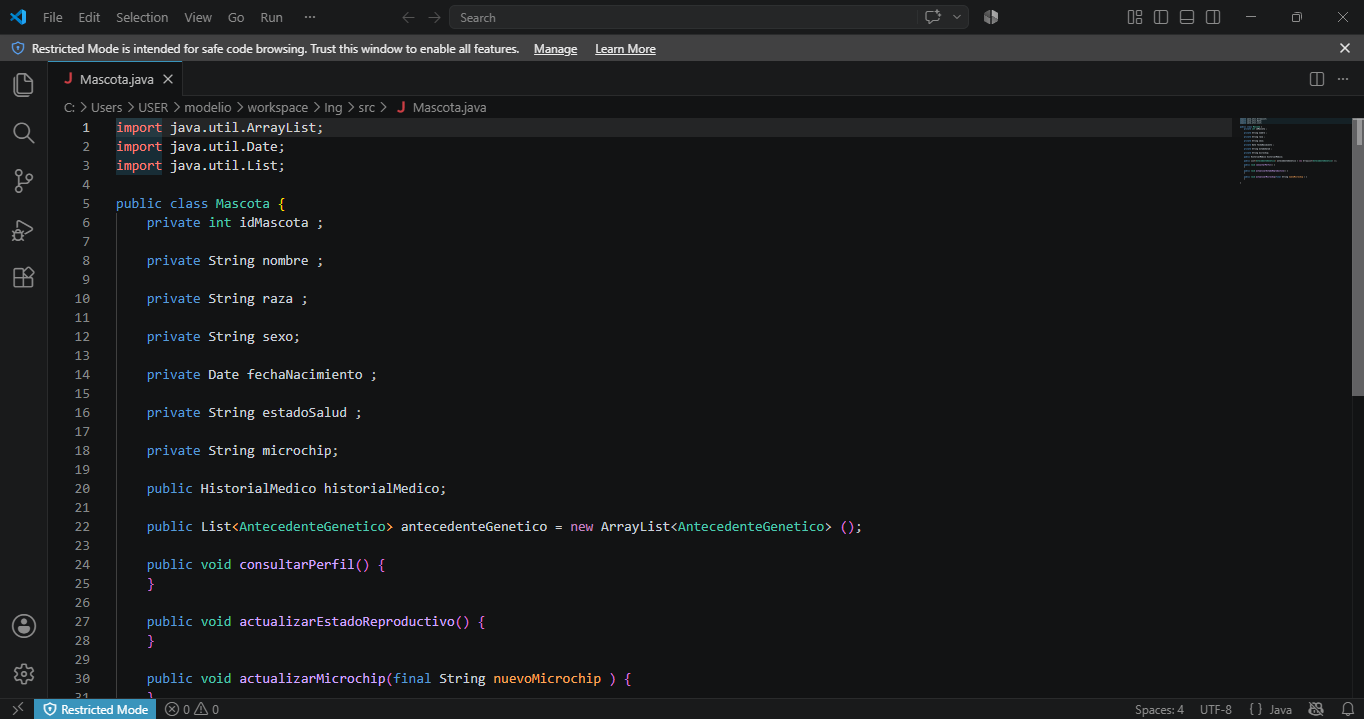
\includegraphics[width=\linewidth]
			{figuras/roundtrip_codigo_despues.png}
			
			\small (b) Código después de la regeneración.
		\end{minipage}
		
		\caption{Comparación del código Java antes y después de la
			regeneración.}
		\label{fig:anexo-roundtrip-codigo}
	\end{figure}
	
	%==================================
	% ANEXO: GITHUB
	%==================================
	
	\section{Repositorio GitHub}
	
	El repositorio público utilizado para almacenar el modelo, código,
	documentación y evidencias se encuentra disponible en:
	
	\begin{center}
		\href{
			https://github.com/MoralesGaryUteq/PFC-MundiPets-MDD-EquipoE
		}{
			\texttt{PFC--MundiPets--MDD--EquipoE}
		}
	\end{center}
	
	\subsection{Estructura del repositorio}
	
	\begin{figure}[H]
		\centering
		\footnotesize
		\begin{verbatim}
			PFC-MundiPets-MDD-EquipoE/
			|-- README.md
			|-- docs/
			|   |-- informe.tex
			|   |-- informe.pdf
			|   |-- referencias.bib
			|   `-- figuras/           (diagramas y capturas)
			|-- modelo/
			|   |-- Ing.zip            (proyecto nativo de Modelio)
			|   `-- perfiles/          (perfil UML aplicado)
			|-- plantillas/
			|   `-- README.md (justificación de la plantilla/configuración)
			|-- codigo-generado/
			|   `-- *.java             (8 clases generadas)
			|-- evidencias/
			|   `-- capturas/          (generación, compilación, verificación)
			|-- exposicion/
			|   |-- diapositivas.pdf
			|   `-- README.md          (enlace al video)
			`-- borradores/
				|-- MoralesGary/
				|   `-- BorradorMoralesSanchezGaryAlejandro.pdf
				`-- NievesJimmy/
			     	`-- BorradorNievesSanchezJimmySamuel.pdf
		\end{verbatim}
		\caption{Estructura general del repositorio del proyecto.}
		\label{fig:anexo-github-repositorio}
	\end{figure}

	
	\subsection{Historial de commits}
	
	\begin{figure}[H]
		\centering
		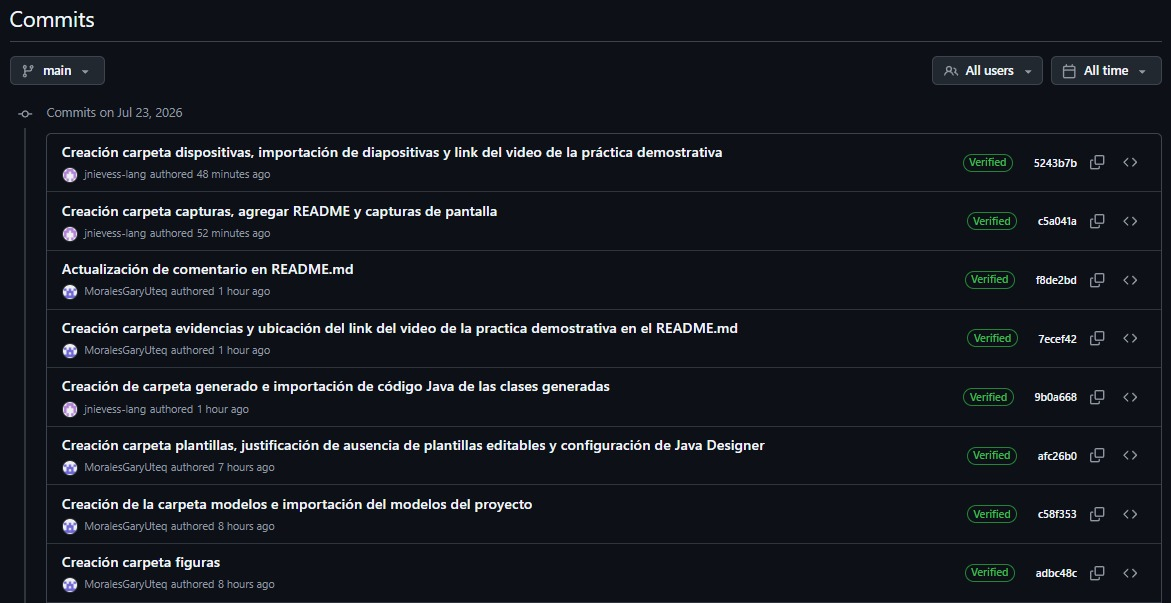
\includegraphics[width=0.94\textwidth]
		{figuras/github_commits.jpeg}
		\caption{Historial de commits realizados durante el desarrollo.}
		\label{fig:anexo-github-commits}
	\end{figure}
	
	\subsection{Participación de los integrantes}
	
	\begin{figure}[H]
		\centering
		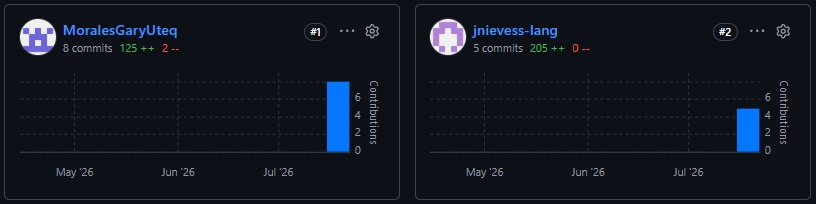
\includegraphics[width=0.90\textwidth]
		{figuras/github_contributors.jpeg}
		\caption{Contribuciones registradas por los integrantes del equipo.}
		\label{fig:anexo-github-contributors}
	\end{figure}
	
\end{document}